%----------------------------------------------------------------------------
% ----- File:        ut1lib.tex 
% ----- Author:      Rainer Menzner (rmz@neuroinformatik.ruhr-uni-bochum.de)
% ----- Date:        2000-01-03
% ----- Description: This file is part of the t1lib-documentation.
% ----- Copyright:   t1lib is copyrighted (c) Rainer Menzner, 1996-2000. 
%                    As of version 0.5, t1lib is distributed under the
%                    GNU General Public Library License. The
%                    conditions can be found in the files LICENSE and
%                    LGPL, which should reside in the top level
%                    directory of the distribution.  Please note that 
%                    there are parts of t1lib that are subject to
%                    other licenses:
%                    The parseAFM-package is copyrighted by Adobe Systems
%                    Inc.
%                    The type1 rasterizer is copyrighted by IBM and the
%                    X11-consortium.
% ----- Warranties:  Of course, there's NO WARRANTY OF ANY KIND :-)
% ----- Credits:     I want to thank IBM and the X11-consortium for making
%                    their rasterizer freely available.
%                    Also thanks to Piet Tutelaers for his ps2pk, from
%                    which I took the rasterizer sources in a format
%                    independ from X11.
%                    Thanks to all people who make free software living!
%----------------------------------------------------------------------------

\newpage
\section{Using \tonelib}
This section describes in detail how to use \tonelib. I have tried to
to describe the stuff in the order a new user would learn best and a new user
would need to use the functions. 


\subsection{Compiling and Linking \tonelib-Programs}
\label{compilingprograms}%
A program that wants to use functions from the library must include
the appropriate headers at compile time and then be linked with the
appropriate libraries. Since V. 0.6-beta the X11 interface is separated
from the \tonelib\ pivotal stuff. This yields advantages for programs that
don't use the X11 rastering functions on systems where X11 is
installed. 
The following applies to programs that do not use the X11 rastering
functions: 
\begin{itemize}
\item Include the file \verb+t1lib.h+. All definitions and declarations
  needed at compile time are included in this file.
\item \verb+libt1.a+ or \verb+libt1.so+ respectively must be linked to the
  program. 
\end{itemize}
In contrast, a program that uses the X11 interface must adhere to the
following scheme:
\begin{itemize}
\item \verb+t1lib.h+ and \verb+t1libx.h+ must be included in this
  order. Furthermore, \verb+t1libx.h+ includes \verb+X11/Xlib.h+ if
  it is not already included.
\item The libraries \verb+libt1.a+/\verb+libt1.so+ and
  \verb+libt1x.a+/\verb+libt1x.so+ must be linked to the executable. 
  The correct order is \verb+-lt1x -lt1+ since the X interface uses
  functions from the latter. Also, the X11 library must appear in the
  library list after \verb+-lt1x+.
\end{itemize}
The Makefiles for \verb+xglyph+ and \verb+type1afm+ are typical
examples for both configurations.


\subsection{Querying and Setting Fundamental Configuration Parameters of \tonelib}
\label{queryconfiguration}%
It might be necessary to know whether \tonelib\ is compiled with or without
X11 interface. At compile time a programmer can check for the X11 interface by
stating
\begin{verbatim}
#ifdef T1LIB_X11_SUPPORT
\end{verbatim}
after including \verb+t1libx.h+. If \verb+T1LIB_X11_SUPPORT+ is not defined,
the X11 interface is not configured and compiled.

At runtime, a program can check for the X11 interface by a call to 
\precorr
\begin{verbatim}
 int T1_QueryX11Support( void)
\end{verbatim}\index{\verb+T1_QueryX11Support()+}\postcorr
It returns \verb+1+ if the X11 interface is present and \verb+0+ otherwise.

Notice that querying X11 support at runtime and compile time tends to
be pretty useless starting with V.~0.6-beta. Any decision can be done
by examining the existence of the \verb+t1x+-library and the
\verb+t1libx.h+ header file. The definition and the function described
above are thus only provided for compatibility with pre-0.6 versions
of \tonelib. 

Some remarks on the general data format of bitmaps and should be given
here. \tonelib\ internally always generates bitmaps in the way that appears to
be natural for them: The first pixel corresponds to the least significant bit
in a byte (or word/longword). Bytes are always arranged in memory the way,
that the first byte is at the lowest address and the next byte at the
following address. This convention is called LSBFirst which stands for Least
Significant Bit/Byte First. It is the natural way of data alignment on
machines with {\em Little Endian} data representation. In contrast MSBFirst
stands for Most Significant Bit/Byte First which is the natural kind of data
representation on Big Endian machines. 
A glyph's scanlines are always aligned in LSBFirst-type, no matter on what
machine \tonelib\ is running.  

What has been said above, strictly does only apply to non antialiased glyphs,
i.e., real bitmaps. Antialiased glyphs have their gray values coded in the
representation that is natural for the machine \tonelib\ is running on. For
example, if \tonelib\ runs on a Big Endian machine, the gray values are in Big
Endian. The X11 displaying functions automatically handle this correct.

Scanlines of \tonelib-glyphs may be padded to 8, 16 or 32 bit. Padding to
higher values will consume more memory for the glyphs, but might speed up
concatenating of bitmaps as described in \ref{generatingbitmaps}. This applies
to machines with Little Endian representation as, for example, Intel's 
$x$86 series. On these machines 16 or 32 bits can be placed into the
target bitmap in one step. On machines with Big Endian representation, for
example, Motorola 680$x$0 series, this is currently not possible. However,
using a higher padding value could still yield a better performance since the
application could work on larger units than a byte.

The default padding value in \tonelib\ is 8 bit. The padding value can be
specified at runtime by means of calling  
\precorr
\begin{verbatim}
 int T1_SetBitmapPad( int pad)
\end{verbatim}\index{\verb+T1_SetBitmapPad()+}\postcorr
\verb+pad+ must be one of `8', `16' or `32'. The call will only be successful
if executed before initialization of \tonelib. This a security mechanism which
prevents from having glyphs with distinct padding values. The return value is
0 if successful and -1 if \verb+pad+ was invalid or \tonelib\ had already been
initialized.

There is a further restriction concerning the padding value. Setting it to 32
is only possible if the machine has an ANSI C integer type of 64 bits. This
condition is automatically checked by the \verb+configure+ script of \tonelib.
If such an integer type is not present (or has to be emulated as e.g.\ 
\verb+long long+ in \verb+gcc+) there would not result any performance gain.
If a specified padding value is rejected, \verb+T1_errno+ is set
appropriately. 

An application can query the current padding value by calling 
\precorr
\begin{verbatim}
 int T1_GetBitmapPad( void)
\end{verbatim}\index{\verb+T1_GetBitmapPad()+}\postcorr
The returned value is the padding value. This function can be called before or
after initialization of \tonelib.

Another function usually be called near
initialization is
\precorr
\begin{verbatim}
 int T1_SetDeviceResolutions(float x_res, float y_res) 
\end{verbatim}\index{\verb+T1_SetDeviceResolutions()+}\postcorr
This function allows setting the resolution of
your device (screen). The values must be given in dpi. The default
resolution, 72 dpi, implies that a pixel in device space equals 1
bp. This function may be called before or after initialization. The
only restriction is that no size dependent data must be
available. Changing the resolution when bitmaps are already cached would 
result in inconsistent bitmap-sizes for bitmaps generated before and
after the call to \verb+T1_SetDeviceResolutions()+.
The function checks whether initialization has already been done. If
not, all is OK since no size-dependent data for any font can exist. If
initialization has been done, it checks for every font whether size
dependent data exists. If there's any size dependent data for any
font, \verb+T1_SetDeviceResolutions()+ will return \verb+-1+ without
having set the new resolution. Otherwise the specified resolution will
be set and the function will return \verb+0+.
If you really need to set
another resolution in the middle of a session, all size-specific data
should explicitly be removed from memory beforehand. This can be
achieved using \verb+T1_DeleteAllSizes()+ (see \ref{deletingdata}).

Notice that the device resolution need not be set at all if the default
resolution of 72 dpi in horizontal and vertical direction is OK. This function
is primarily intended to be prepared for applications with a device aspect
ratio different from 1.
 
\subsection{Initialization of \tonelib\ and Related Things}
\label{initialization}%
In this section we should cover the initialization, part of which has already
been described in \ref{runtimesetup} in some more detail. This gives the user
the chance to fine-tune the initialization for specific applications.

Prior to be able to do anything useful with \tonelib, the library has to be
initialized. Generally speaking, the purpose of the initialization is to tell
\tonelib\ which font files are associated with which font ID's. The existence
or accessibility of the font files is also assured at this point. Hence, file
name search paths for Type 1 font files, AFM files and encoding files have
also to be known at this time. 

The configuration file and the font database file play a central  r\^ole
during initialization. While the configuration file contains path
specifications and a font database specification, the font database file
specifies the relation between font ID's and font filenames.
The format of both these files is described in \ref{runtimesetup} and not
repeated here. 

A further purpose of the initialization is to set certain flags that prevent
other quantities from being modified at a later time. For example, the padding
value must be unique to all glyphs and consequently it is not allowed to be
changed after initialization has been performed.

The initialization is started by a call to the function
\precorr
\begin{verbatim}
 void *T1_InitLib( int log)
\end{verbatim}\index{\verb+T1_InitLib()+}\postcorr
The parameter \verb+log+ can be interpreted as a mode specification that
influences certain parts of the initialization.  In fact it should consist of
one or more \verb+#define+s from \verb+t1lib.h+.  At minimum, \verb+log+
should be either \verb+LOGFILE+ or \verb+NO_LOGFILE+. If \verb+LOGFILE+ is
specified, a log file is written while the application runs, and
\verb+NO_LOGFILE+ suppresses the generation of a logfile. For information the
\tonelib-logfile see \ref{logfile}.  In addition to this,
\verb+IGNORE_CONFIGFILE+ and \verb+IGNORE_FONTDATABASE+ can be bitwise OR'ed
(using ``\verb+|+'') to the \verb+log+-value. The purpose of this is described
later in this section. A further flag that might find its way into the value
of \verb+log+ is \verb+T1_AA_CACHING+. A discussion of this topic is given in
\ref{aacaching}.
The \verb+T1_NO_AFM+ completely suppresses usage of AFM data, no matter if an
AFM file could have been found using the current search paths or not. This
saves time for loading a font and is recommended if an application is known to
be restricted on functions that do not access AFM data. The consequences of
using this flag are covered somewhat more detailed in \ref{generatingafminfo}.


\subsubsection{Standard Initialization}
\label{standardinitialization}%
The term ``standard initialization'' means, that none of the path manipulating
and font database manipulating actions described later has been
performed. Also, a standard initialization excludes the use of
\verb+IGNORE_CONFIGFILE+ and \verb+IGNORE_FONTDATABASE+. If these conditions
are met, the following happens at initialization time:
\begin{enumerate}
\item The padding value, either being the default value or a value specified
  by the user before, is assigned.
\item Next, depending on the value of \verb+log+, a logfile is tried to be
  opened. From this point on, depending on the loglevel and the value of
  \verb+log+ the actions are logged.
\item The endianess of the machine \tonelib\ is running on is checked. 
\item A configuration file is searched in the following order:
  \begin{itemize}
  \item The process' environment is checked for the entry \verb+T1LIB_CONFIG+
  and if found, its value is interpreted as the filename of the configuration
  file (see \ref{runtimesetup}).
  \item If no file was found, the user's home directory is searched for a file
    named \verb+.t1librc+. In case it exists, it is used as a
    \tonelib-configuration file. 
  \item If still no configuration file was found, the global configuration
    file will be tried to be opened.
  \item If this also does not succeed, all file search paths are left to be
    ``.'' and the default font database is \verb+FontDataBase+.
  \end{itemize}
  It should be noted that the first match wins when searching the configuration
  file. Only the first one found is examined.
\item The font database file is tried to be opened and is read. This process
  is in detail described in \ref{fontdatabase}. Note that you cannot count on
  the assignment of the ID's in last resort. A font in line 10 of the font 
  database file will only get font ID 8 if for all preceding lines the font
  file could be located. Otherwise, the font ID will be correspondingly
  smaller. 

  If a fatal error occurs while processing the font database file,
  \verb+T1_InitLib()+ will immediately return with a \verb+NULL+ pointer
  indicating the initialization has failed. 
\item The number of fonts declared in the database is stored. Note that this
  number of declared fonts may also be 0.
\item A flag is set to indicate \tonelib\ is initialized and the pointer to
  the top most area of the global data structures is returned to the
  application. This pointer is guaranteed to be not \verb+NULL+.
\end{enumerate}
For some applications, the described initialization scheme appears to be too
inflexible and overkill. It is well suited for large applications that use
lots of fonts and where it should be possible to add new fonts without
modifying the application itself. For small commandline applications like
\verb+type1afm+ (see \ref{type1afm}), which are designed to read a few font file
names from the commandline, the overhead in configuration file searching and
path reading is much too large. Moreover, to insist on a font database file
might grow to a real disadvantage. In the subsequent paragraphs we should thus
discuss how we can deviate from the initialization scheme described above.

\subsubsection{Setting Font Database and File Search Paths}
\label{manipulatingpaths}%
First, it is important to mention that it is generally possible to force
\verb+T1_InitLib()+ to skip steps 4 and 5 as described above. 

The configuration file is discarded by OR'ing the parameter \verb+log+ of
\verb+T1_InitLib()+ with \verb+IGNORE_CONFIGFILE+. The default paths or the
paths explicitly specified by the application before are conserved during
initialization. 

Discarding the font database explicitly is achieved by bitwise OR'ing
\verb+log+ with \\ 
\verb+IGNORE_FONTDATABASE+. The result after initialization
will be an empty database. This is valid in V.\ 0.5 and newer since fonts may
be added to the database at runtime. 

An alternative to discarding the whole configuration file is to selectively
overwrite or discard the entries contained therein. The font database may
explicitly be specified by the application using 
\precorr
\begin{verbatim}
 int T1_SetFontDataBase( char *filename)
\end{verbatim}\index{\verb+T1_SetFontDataBase()+}\postcorr
\verb+filename+ is the pointer to a string containing the name of the font
database file that is to be examined. This function is to be called before
\verb+T1_itLib()+. When the configuration file is examined during
initialization, it is checked whether a font database filename has explicitly
been set. And if so, the entry in the configuration file is discarded and the
explicitly specified font database file is examined later.

A similar manipulation is possible for the searchpaths. This is done by
calling 
\precorr
\begin{verbatim}
 int T1_SetFileSearchPath( int type, char *pathname)
\end{verbatim}\index{\verb+T1_SetFileSearchPath()+}\postcorr
before calling \verb+T1_InitLib()+. An attempt to set the file searchpaths
after \verb+T1_InitLib()+ has been called is denied. The reason is that it is
not wise to override the searchpaths which have been valid at initialization
time since those paths have been examined to verify the existence of font files
during initialization. These paths should thus not be removed. 
The parameter \verb+pathname+ points to the string that contains the pathname
that should be used as searchpath. The parameter \verb+type+ is any
OR'ed combination of \verb+T1_PFAB_PATH+, \verb+T1_AFM_PATH+ and
\verb+T1_ENC_PATH+. These tell the function to set the search paths for Type 1
font files, AFM files and encoding files, respectively. In case of an error
\verb+-1+ is returned and otherwise \verb+0+.

Extending the file searchpaths before {\em and} after initialization
is possible using 
\precorr
\begin{verbatim}
 int T1_AddToFileSearchPath( int pathtype, int mode, char *pathname)
\end{verbatim}\index{\verb+T1_AddToFileSearchPath()+}\postcorr
This might be useful to locate font files that were of no interest
during initialization. 
\verb+pathname+ is the pointer to the string that should be added to the
searchpaths. What searchpaths are affected is determined by the parameter
\verb+pathtype+. Again, similar to described above, any
OR'ed combination of \verb+T1_PFAB_PATH+, \verb+T1_AFM_PATH+ and
\verb+T1_ENC_PATH+ is valid. There are two ways to extend an existing
searchpath which are specified by the \verb+mode+ parameter. It must be either
\verb+T1_APPEND_PATH+ or \verb+T1_PREPEND_PATH+, which causes the new path
element to be appended or prepended to the existent path respectively.
Since an existent path specification is not overwritten by
\verb+T1_AddToFileSearchPath()+, this function may be called at any time
before or after initialization.

It might also be of interest to query the current file search
paths. \tonelib\ provides 
\precorr
\begin{verbatim}
 char *T1_GetFileSearchPath( int type)
\end{verbatim}\index{\verb+T1_GetFileSearchPath()+}\postcorr 
for querying search paths. Again, the parameter \verb+type+ determines
what search path is returned. Exactly one of \verb+T1_PFAB_PATH+,
\verb+T1_AFM_PATH+ and \verb+T1_ENC_PATH+ should be specified. If more
than one path is specified, the first match wins and only one path is
returned. The first will be in the order \verb+T1_PFAB_PATH+,
\verb+T1_AFM_PATH+ and \verb+T1_ENC_PATH+. 


\subsubsection{Adding Fonts to the Database} 
\label{addingfonts}%
Extending the font database is possible at any time after initialization. It
is done via a call to 
\precorr
\begin{verbatim}
 int T1_AddFont( char *fontfilename)
\end{verbatim}\index{\verb+T1_AddFont()+}\postcorr
\verb+fontfilename+ is the pointer to the filename string. The following
actions take place:
\begin{itemize}
\item The font file is searched using the current search path specifications. 
\item If the file has been located, it is checked whether the font database
  contains enough memory to hose an additional font. 
  If so, the font filename
  is stored and the function returns \verb+new_ID+, which is the font ID that
  will be associated with this font in the future. 
\item If there was no free memory for an additional font, the memory is
  reallocated to a greater size. This involves also resetting the new
  area. Finally the value \verb+new_ID+ is returned.
\end{itemize}
If a negative value is returned the function failed. \verb+-1+ indicates the
font file could not be located. \verb+-2+ or \verb+-3+ are returned if a
memory allocation failure occurs.


\subsubsection{Bypassing the \tonelib\ File Search Machinery} 
\label{afmfilenames}%
Usually, \tonelib\ takes care for locating files according to the path
specifications in the configuration file. There might, however, arise the need
to explicitly tell \tonelib\ which particular file to use. Forcing \tonelib\ to
use particular Type 1 font files can be achieved using the function
\verb+T1_AddFont()+, described just above. If a pathname passed to this
function is a complete path, \tonelib\ will use this complete path to locate
the font file, forgetting about its own search path list. A filename path is
assumed to be complete if 
\begin{itemize}
\item it starts with the directory separator character, usually
  ``\verb+/+''. In this case it is an {\em absolute} path specification, meaning
  that the start point is at the root of the filesystem, or
\item if it starts with ``\verb+./+'' or ``\verb+../+'' (where it is assumed
  that ``\verb+/+'' is the directory separator character). Here we have a {\em
    relative} path specification in which ``\verb+.+'' refers to the current
  working directory while ``\verb+..+'' refers to the parent directory of the
  current working directory. Since the notion of the {\em current working
    directory} is fundamental for every process that has access to a
  filesystem, a relative path specification also uniquely identifies one
  particular file in the filesystem.
\end{itemize}
If a font file whose complete path had been specified could not be found by
\tonelib, the paths from the configuration file are searched as a fallback
mechanism. 

What can be done for the Type 1 font files is also possible for AFM files,
which are needed on a per-font basis. The function
\precorr
\begin{verbatim}
 int T1_SetAfmFileName( int FontID, char *afm_name)
\end{verbatim}\index{\verb+T1_SetAfmFileName()+}\postcorr
allows to set the complete path of the AFM file belonging to the font
identified by \verb+FontID+, overriding the internal
search mechanism. This function is to be called after initialization but
before the font \verb+FontID+ is loaded. It returns 0 if all goes right and
$-1$ otherwise. In the latter case \verb+T1_errno+ will also be set
appropriately. Notice that \verb+FontID+ must also be valid with respect to
its upper limit, it is an error condition if the font database has less than
\verb+FontID+ entries. 

There is also the function 
\precorr
\begin{verbatim}
 char *T1_GetAfmFileName( int FontID)
\end{verbatim}\index{\verb+T1_GetAfmFileName()+}\postcorr
which allows to query the AFM filename of a font. It returns a pointer to the
filename if it had explicitly been specified or \verb+NULL+
otherwise. \verb+NULL+ will also be returned if \verb+FontID+ was invalid. In
this case also \verb+T1_errno+ will be set.  

Just for the sake of completeness we should mention that what has been said 
about absolute and relative path specification
also applies to pathnames for encoding files (see \ref{encoding}).




\subsection{The \tonelib-Logfile}
\label{logfile}%
Since version 0.2-beta \tonelib\ supports a runtime logfile.
It implements an uncomplicated way to keep track of errors,
warnings, statistics and debug messages without overloading stdout/stderr. As
seen in \ref{initialization} the user must specify whether or not to use a
logfile when calling \verb+T1_InitLib()+. Specifying \verb+LOGFILE+ as
argument leads to using a logfile and \verb+NO_LOGFILE+ suppresses the use of a
logfile.

The name of this logfile is by default \verb+t1lib.log+. This name is defined
in \verb+t1misc.h+ and can be changed there as the user likes.

Basically \tonelib\ distinguishes 4 types of runtime messages. Each type is
associated a ``loglevel'':
\begin{itemize}
\item {\sl Errormessages/Level1:}\/ They are considered that important that the user is
  in any case informed. Example: During initialization the memory allocation for
  one of the basic data structures of \tonelib\ failed.
\item {\sl Warningmessages/Level2:}\/ They are considered important but it is not
  absolutely necessary to inform the user. Example: An AFM file could not be
  loaded for a given font. This imposes several restrictions on what can be
  done with that font but it is possible to generate bitmaps.
\item {\sl Infomessages/Level3:}\/ They do not indicate a problem. Rather, the user
  is notified about some facts and statistics that might be of
  interest. Example: After loading a font the consumption of virtual memory is
  displayed. 
\item {\sl Debugmessages/Level4:}\/ These can be pointers, numerical data
  etc. Example: Print out the pointers that point to the memory area where the
  PostScript dictionaries for a font just loaded are located.
\end{itemize}
The decision what message to put into the logfile is done by examining the
value of an integer variable whose values can be \verb+T1LOG_ERROR+ (=1),
\verb+T1LOG_WARNING+ (=2), \verb+T1LOG_STATISTIC+ (=3) or \verb+T1LOG_DEBUG+
(=4). All messages whose level is below or equal to this value are put into the
logfile. The user may set this loglevel by calling
\precorr
\begin{verbatim}
 void T1_SetLogLevel( int level)
\end{verbatim}\index{\verb+T1_SetLogLevel()+}\postcorr
The default value is \verb+T1LOG_WARNING+ which means that error and warning
messages are stored in the logfile. 

If the usage of a logfile has been specified, \tonelib\ tries first to open
it in the current directory. If this fails for some reason \tonelib\ tries
to create it in the user's home directory. If this fails too, an error message
is printed to stderr and no logfile is used.

The user himself may also put some messages into the logfile. This can be
achieved using
\precorr
\begin{verbatim}
 void T1_PrintLog( char *func_ident, char *msg_txt, int level)
\end{verbatim}\index{\verb+T1_PrintLog()+}\postcorr
where \verb+func_ident+ is a pointer to a string identifying the function that
generates the message. \verb+msg_txt+ points to the text string to put
out. The distinction between a function identifier and a message text is only
formal, indicating the user should identify the function that generates the
message. 

If values are to be put in, \verb+msg_txt+ has to be created with
\verb+sprintf()+, for example. The \verb+level+ specification works as
described above: The message is only put out if the internal loglevel is
equal or greater than \verb+level+. 

Here is a typical example of a log file after a (short)
\verb+xglyph+-session in which the loglevel was set
\verb+T1LOG_STATISTIC+. Among several informative messages of type S, also two
messages of type W have been generated. They stem from trying to
raster the character ``\ss'' which was not in the current encoding. 
\par\noindent
{%
\tiny
\begin{verbatim}
(S) (Mon Jul 14 18:27:34 1997) T1_InitLib(): Initialization started 
(S) (Mon Jul 14 18:27:34 1997) T1_InitLib(): Initialization succesfully finished 
(S) (Mon Jul 14 18:27:44 1997) T1_LoadFont(): VM for Font 0: 35132 bytes 
(S) (Mon Jul 14 18:27:44 1997) CreateNewFontSize(): New Size 100.000000 created for FontID 0 (antialias=0) 
(S) (Mon Jul 14 18:27:53 1997) CreateNewFontSize(): New Size 100.000000 created for FontID 0 (antialias=1) 
(S) (Mon Jul 14 18:27:53 1997) CreateNewFontSize(): New Size 200.000000 created for FontID 0 (antialias=0) 
(W) (Mon Jul 14 18:27:53 1997) T1_SetChar(): No black pixels found for character 223 from font 0, returning NULL 
(W) (Mon Jul 14 18:27:53 1997) T1_SetStringX(): T1_SetChar() returned NULL-pointer! 
(S) (Mon Jul 14 18:27:55 1997) T1_DeleteSize(): Size 200.000000 deleted for FontID 0 (antialias=0) 
(S) (Mon Jul 14 18:27:55 1997) T1_DeleteSize(): Size 100.000000 deleted for FontID 0 (antialias=0) 
(S) (Mon Jul 14 18:27:55 1997) T1_DeleteSize(): Size 100.000000 deleted for FontID 0 (antialias=1) 
\end{verbatim}
}

\subsection{Generating Bitmaps}
\label{generatingbitmaps}%
At this point, you are able to generate a bitmap.
As said before, a character- or string-bitmap is given to the user as
an object of type \verb+GLYPH+. We should briefly explain \verb+GLYPH+
here. The type is defined by
\begin{verbatim}
typedef struct
{
  char *bits; 
  struct          
  {
    int ascent;
    int descent;
    int leftSideBearing;
    int rightSideBearing;
    int advanceX;
    int advanceY;
  } metrics;
  void *pFontCacheInfo;
  unsigned long bpp;
} GLYPH;
\end{verbatim}
\verb+bits+ is a pointer to the bitmap data. The
bitmap is organized in lines, starting with the uppermost line.
Each bitmap pixel is usually represented by one bit. If the width of
the 
bitmap is not an integer multiple of 8, the lines are padded with
zeros, so that each line starts at a byte boundary. Note that the
bitmap has no margins taken into account. The bitmap occupies the
minimum area the character needs to be painted. 

The bitmap pointer may also be
the \verb+NULL+-pointer. In this case, the glyph contains no foreground
pixels. The metrics of the corresponding glyph should be valid,
though. Typically, this appears for the space character as well as in
situations where an undefined or unencoded character had been substituted by
the \verb+.notdef+-character within the rastering functions.

Note that the \verb+pixmap+-entry which has been present in version 0.3-beta,
has been removed with version 0.4-beta. See the discussion on the X11-interface
in \ref{x11interface} for an explanation of this.

The struct \verb+metrics+ contains metric information that is needed
to position the character and to describe the character origin
with respect to the bitmap. The members in detail:
\begin{itemize}
\item \verb+metrics.ascent+: describes how many lines the bitmap
  ranges above the line $y=0$. 
\item \verb+metrics.descent+: describes how many lines the bitmap
  ranges below the line $y=0$. Width below $y=0$ counts negative so that the
  difference \verb+ascent+ $-$ \verb+descent+ is the
  total height of the bitmap, the number of lines.
\item \verb+metrics.leftSideBearing+: The amount of spacing between
  the origin of a character and the x-coordinate of its leftmost
  painted pixel. One could also name it ``left margin'' of the
  character. 
\item \verb+metrics.rightSideBearing+: The horizontal difference between
  the origin of a character and the x-coordinate of its rightmost
  painted pixel. This definition stands in contrast to some other
  interpretations of the right side bearing, where it is assumed as the
  difference between the glyph's width and its right most pixel.
\item \verb+metrics.advanceX+: The amount of position increment in
  horizontal direction after this character
  bitmap (or string bitmap) has been placed. It is almost always
  larger than the bitmap width because most characters contain a
  certain amount of margins. Note that this value is not suitable for internal
  computations of character positions since it contains the horizontal
  escapement rounded to the pixel grid. Using this value for such computations
  leads to accumulating positioning errors.
\item \verb+metrics.advanceY+: The amount of position increment in
  vertical direction after this character
  bitmap (or string bitmap) has been placed. Upper direction counts positive. 
\end{itemize}
As seen, the width of the bitmap is given as the difference between
\verb+rightSideBearing+ and \verb+leftSideBearing+ and the values
\verb+metrics.leftSideBearing+, \verb+metrics.descent+,\\
\verb+metrics.rightSideBearing+ and \verb+metrics.ascent+ effectively describe
the bounding box of the glyph.

The entry \verb+pFontCacheInfo+ is not currently used but will
probably later when font caching is really
implemented. Moreover, there's a certain chance that some other
entry will be added in future releases.

The member \verb+bpp+ is used to store the depth of the bitmap. For
true bitmaps, it is always 1. See \ref{antialiasing} for an
explanation. 

There are two functions which produce pointer to glyph objects. In
order to generate the glyph for a single character you would use the
function 
\precorr 
\begin{verbatim}
 GLYPH *T1_SetChar( int FontID, char charcode, 
                    float size, T1_TMATRIX *transform)
\end{verbatim}\index{\verb+T1_SetChar()+}\postcorr
As in most other functions, \verb+FontID+ is a valid identification
number of a font. It can range from 0 to $n-1$, where $n$ is number of
fonts declared in the font database file.

The second argument \verb+charcode+ determines the character that will
be rasterized.
As mentioned earlier, the encoding mechanism is used for
accessing the output character. This means, if \verb+'A'+ is given as
the character code, the machine representation of \verb+'A'+ is used
as an index into the current encoding vector. In this encoding vector,
the characters' name is looked up. Encoding vectors may be changed by
the user (see \ref{encoding}).


The parameter \verb+size+ is interpreted in Postscript's bigpoint-unit
(bp). By default, 
1 bp equals one device pixel. 

\verb+transform+ specifies the transformation that will be applied to the
character before rastering. If this pointer is \verb+NULL+, no transformation
is used. Otherwise it should point to a valid \tonelib-transformation matrix.
Please refer to \ref{transformations} for information on how to easily create
\verb+T1_TMATRIX+ matrices.
Hinting is only performed if the transformation is a pure rotation and if the
the angle is one of 0, 90, 180 or 270 degrees. Otherwise font level and
character level hinting information is ignored.

Bitmaps of transformed characters are never saved in
cache memory since I assume that they are rarely needed. The overhead
to manage transformed characters in cache would be overkill and would
significantly increase memory consuming. Anyhow, this would only work
for some dedicated transformations.

\verb+T1_SetChar()+ in fact does some more things than simply
rastering the specified character:
\begin{itemize}
\item It checks whether the font in question is already loaded. If not,
  it is loaded. 
\item If the size dependent data structures for the size in question
  do not exist, it creates them and inserts them in the linked list of
  size dependent data structures.
\item It checks if the character is already existent in cache. If so,
  it returns the data from cache.
\end{itemize}

Some words concerning memory management: The memory used by
the \verb+GLYPH+-structure is static in this function. The memory
required for the bitmap is also allocated by the function itself.
This means, the user doesn't need to free any memory by
himself. Every time \verb+T1_SetChar()+ is called, it starts by giving the
memory needed for the last generated glyph free or respectively
setting metric values to 0. Thus, do not free the
returned glyph pointer since later \verb+T1_SetChar()+ will free
memory that is no more allocated and probably used for some other purpose.
If you really like to free the memory, set the pointer to \verb+NULL+
afterwards. 

If an error occurs at some point, \verb+T1_SetChar()+ returns a
NULL-pointer to the user.

Frequently it is advantageous to raster a series of
characters at once. This has the advantage that internal accuracy may
be used and the overhead for the user is minimal. For such cases, the
function 
\precorr
\begin{verbatim}
 GLYPH *T1_SetString( int FontID, char *string, int len, 
                      long spaceoff, int modflag, 
                      float size, T1_TMATRIX *transform)
\end{verbatim}\index{\verb+T1_SetString()+}\postcorr
is provided.
It can be considered an extended version of \verb+T1_SetChar()+. The
same as said above applies to the arguments \verb+FontID+,
\verb+size+ and \verb+transform+. But a few additional arguments are
needed here. 

\verb+string+ is a series of bytes representing the indices into the current
encoding vector. 
The \verb+len+-parameter is needed because we cannot imply that string
is always an object like a string in C. For example, the Computer
Modern Roman fonts contain the uppercase Greek Gamma (\char0) at
position 0 in their internal encoding. In a string to be typeset the
value 0 is thus a valid value and deserves no special
treatment. Hence, we cannot not use the C-function \verb+strlen()+ to
compute the length of the string. However, since in most usual encodings
the special value 0 is not encoded (``\verb+.notdef+''), it makes
sense to switch between 
standard situations and non-standard situations:
\begin{itemize}
\item If \verb+string+ is a string conforming with C-semantics,
  \verb+len+ can be set to 0. Then, the length of the string is
  internally computed.
\item If \verb+string+ contains one or more control characters which make
  processing impossible, the \verb+len+-value must be specified
  explicitly. 
\end{itemize}

The \verb+spaceoff+ parameter is important for word processing
purposes. The value specified here is interpreted as an offset to the
space width used during rastering. It is interpreted in charspace
units, i.e., $1/1000$ bp. Every time a space character is requested,
this amount of horizontal escapement is added to the natural
spacewidth of the current font. Note that the space character itself
is actually not rastered. All requests to the character with the
charactername ``\verb+space+'' are caught by \tonelib\ and converted
to a simple horizontal escapement. For computation of the resulting
spacewidth, the width of the space-character is taken from the
AFM data and merged with the specified offset, which may also be
negative.\footnote{One consequence of this handling is, that---with a
  little tricking---fonts that do not define a space character
  themselves may be used for typesetting. This applies to the
  dc-fonts, which only define a visible space, but no real space (see
  \ref{fonts}).}

The \verb+modflag+ argument may be used to specify some option to the
rastering function. It is generally 0 or an OR'ed combination of the following
names:
\begin{itemize}
\item \verb+T1_KERNING+: As the name implies, this argument
  determines that pairwise kerning information from the AFM file is to be taken
  into account during string rastering. Not specifying \verb+T1_KERNING+ 
  means: ``omit kerning''. It is generally
  recommended to use kerning information since this improves the optical
  appearance. However, many lower quality fonts do not have kerning
  information.  With \tonelib\ V.\ 0.4-beta, kerning information is accessible
  much faster than before because it is based on char codes rather than on
  characternames.
\item \verb+T1_RIGHT_TO_LEFT+: Setting this flag will invert the writing
  direction. In {\em Right-To-Left} mode the escapement in writing direction
  (left) is inserted before placing the character with the result that the
  character laps over to the left side. This principle is kept for all
  characters in the string. Note that metrics of fonts that are intended for
  {\em Right-To-Left} typesetting have the same meaning as for fonts intended
  for standard ({\em Left-To-Right}) typesetting.
\item \verb+T1_UNDERLINE+: The string to be rastered is to be underlined
  according to the line specifications of the current font. 
\item \verb+T1_OVERLINE+: The string to be rastered is to be over lined.
\item \verb+T1_OVERSTRIKE+: Same here for overstriking. 
\end{itemize}
For a description of underlining and such, see \ref{underlining}. Notice also
that the \verb+modflag+ argument is a replacement of the \verb+kerning+
argument from pre-0.7 versions of \tonelib.

Concerning glyph-memory considerations, the same applies as said under
the description of \verb+T1_SetChar()+: Never free a pointer to memory
which was returned by \verb+T1_SetString()+. Or, alternatively, if freeing
the pointer cannot be avoided set it to NULL after freeing it.\footnote{For
  example, {\tt XDestroyImage()} gives the pixel memory for the image
  data free although it might not have been allocated by any X11-function.} 

There are two generic ways how a string-glyph can be produced. The first is to
take the paths of all characters needed, concatenate them, insert space and
kerning amounts as needed and raster the resulting whole path. This will yield
the best results since the average position accuracy of the pixels will be
optimal. This applies especially for rotated strings. The drawback is, that
every character must be rastered every time it is needed. There is no way to
access the bitmap data of a character inside a rastered string separate from
others. And the caching of string-glyphs at this programming level doesn't
make any sense. So this principle takes significantly longer than
concatenating bitmaps from a cache area. However, it is done when the
specified rotation angle is not equal to $0^\circ$ or when even further
transformation are to be applied.  This condition should limit the total
number of situations when this happens to an amount we can easily bear.

If the \verb+transform+-argument is \verb+NULL+ we know transformations or
rotation should not be applied and another approach is used. We are then able
to construct the resulting bitmap by adjusting already existent bitmaps into
proper positions.  If a character does not already exist in the cache, it is
generated just the way \verb+T1_SetChar()+ works. The calculation of the
character-bitmap positions in the output bitmap is done with
char space-precision.  Nonetheless, there may be differences in the output
compared with output of the above method. These are caused by the fact that
rounding to pixel accuracy has already been achieved when generating the
character bitmap. Thus, the output of the above principle should always be
better since the positions of the black pixels are rounded with respect to the
whole string, and not with respect to a single character glyph. On the other
hand, concatenating character glyphs takes significantly less time than
rastering a complete string.  Theoretically, differences of up to two pixels
horizontal shift may appear in the output of the two principles. You can
check the effect by running the program \verb+xglyph+. Specify a string of
enough length and raster it at angle $0^\circ$. Then specify a very small
angle from 0 different, say, $0.001^\circ$, and raster the string again with
the new setting. You might find that the representation of the string is a
little different now.

If two glyphs with arbitrary orientation exist,
\precorr
\begin{verbatim}
 GLYPH *T1_ConcatGlyphs( GLYPH *glyph1, GLYPH *glyph2,
                         int x_off, int y_off, int modflag)
\end{verbatim}\index{\verb+T1_ConcatGlyphs()+}\postcorr
can be used to concatenate them. First the size of the resulting glyph is
computed and its metric values are filled. Then, the two glyphs are placed at
their appropriate positions in the newly created bitmap. In order to be able
to work, the following conditions must be met:
\begin{enumerate}
\item Either glyph must be different from \verb+NULL+.
\item Both glyphs must have identical \verb+bpp+-values. If antialiased and
  non-antialiased glyphs are to be concatenated, have a look at
\item There must be enough memory for the new glyph (naturally).
\end{enumerate}
The quantities \verb+x_off+ and \verb+y_off+ describe the $x$- and
$y$-component of an optional offset to be inserted between the two
glyphs. This offset is interpreted as device pixels. The \verb+modflag+
argument is used to specify the direction in which the two glyphs are to be
concatenated. That is, only the bit \verb+T1_LEFT_TO_RIGHT+ /
\verb+T1_RIGHT_TO_LEFT+ is respected by this function.

If problems occur, \verb+NULL+ is returned.
It is generally not recommended to produce large glyphs with this function
because the char space precision in placing the character bitmaps is lost. For
example, three times rounding up an advance by 0.3 pixels accumulates to 1
pixel position error. A similar effect shows up when two rotated and underlined
glyphs are concatenated with this function. There might be a slight shift in the
baseline at the point where the two glyphs touch.

A dilemma occurs, if two antialiased bitmaps have distinct background
colors. Then, it is not clear what the transparent color
is. \verb+T1_ConcatGlyphs()+ always assumes the {\em current} background color
to be transparent.


There is one more function that generates pointers to glyphs:
\precorr
\begin{verbatim}
 GLYPH *T1_CopyGlyph(GLYPH *glyph)
\end{verbatim}\index{\verb+T1_CopyGlyph()+}\postcorr
As mentioned earlier, the user doesn't have the possibility of keeping
the  
glyphs longer than to the next call of the respective rastering function. If 
someone wants to keep a bitmap some time longer,  
\verb+T1_CopyGlyph()+ may be used
to copy the glyph to another area which is then completely under user's
control. This function simply does the following:
\begin{itemize}
\item Allocates the memory for the glyph-structure.
\item If bitmap data is present, it allocates memory for the bitmap data,
  taking the member \verb+bpp+ into account (see \ref{antialiasing}).
\item Copies the structure and the bitmap data to the respective locations.
\item Initializes the pointer \verb+glyph.bits+.
\end{itemize}

Return value is the pointer to the allocated glyph-structure. If something
goes wrong, NULL is returned to indicate an error. A glyph pointer,
returned by a call to this function should be freed by a call to
\verb+T1_FreeGlyph()+ (see \ref{deletingdata}).


\subsection{Loading Fonts Explicitly}
\label{loading}%
Usually there is no need for a user to load a font into memory since this is
done automatically as needed by the rastering functions. But there are two
situations where it makes sense to explicitly load a font before generating
any size dependent data:
\begin{itemize}
\item A font is to be reencoded immediately after loading (see \ref{encoding}).
\item A font is to be transformed (see \ref{transformations}).
\end{itemize}
These operations require a font being loaded but not having any size specific
data. Loading a font explicitly is done by the function
\precorr
\begin{verbatim}
 int T1_LoadFont( int FontID)
\end{verbatim}\index{\verb+T1_LoadFont()+}\postcorr
Loading a font involves several actions:
\begin{itemize}
\item Locating and loading the Type 1 font file.
\item Locating and loading the font metrics data from AFM file.
\item Computing and filling the values of the \verb+FONTPRIVATE+ structure as
  described in section \ref{internals}.
\item Setting up some tables for fast access of metrics information.
\end{itemize}
\verb+T1_LoadFont()+ returns \verb+0+ if successful or \verb+-1+ if the font
could not be loaded. A failure may be due to \tonelib\ not having been
initialized or due to problems with file locations and file parsing. If a font
refuses to load, the logfile should be examined first. Furthermore, in case of
a failure \verb+T1_errno+ will be set appropriately.


\subsection{Functions for Encoding Handling}
\label{encoding}%
As mentioned earlier, the encoding mechanism used in the
PostScript-language allows a font to contain more than 256 different
characters, although only 256 are accessible at a given time. The
characters which are accessible are given by the elements of the
current {\em encoding vector}. In order to maximize flexibility,
\tonelib\ allows for changing the current encoding vector. This is
also called ``Reencoding a font''. A new encoding vector is defined
and made known to the library by creating an encoding-file and loading
its contents into memory. 
Before describing the functions needed for this, we should
briefly describe the format of an encoding file. 

An encoding file is an ASCII text file. No
assumptions about filename extensions are made. Here are the rules for
scanning the file:
\begin{itemize}
\item The file contents are completely ignored until a line is encountered
  that starts with the string \verb+Encoding=+. This string may optionally be
  immediately followed by a string that is assumed to be the identifier of the
  {\em encoding scheme} that this file defines. Any further text on this line
  is ignored.
\item Now, 256 lines have to follow, each line describing one
  character's name. The string ranging from the beginning of the line
  to the first white space character is assumed to be a character
  name. The remainder of the lines is ignored and may (should) be used
  for comments, thereby describing the current character code.
\item All further lines of text are ignored.
\end{itemize}
As well known from PostScript, non-existent characters have to be
named \verb+.notdef+.

Here's an example of such an encoding file:
\begin{verbatim}
Sample encoding file for t1lib!
The first two lines are considered to be comments!
Encoding=ISOLatin1Encoding       
.notdef                          /* '000  000  "00 */ 
.notdef                          /* '001  001  "01 */ 
.notdef                          /* '002  002  "02 */ 
  .                                   .
  .                                   .
  .                                   .
greater                          /* '076  062  "3E */
question                         /* '077  063  "3F */
at                               /* '100  064  "40 */
A                                /* '101  065  "41 */
B                                /* '102  066  "42 */
  .                                   .
  .                                   .
  .                                   .
yacute                           /* '375  253  "FD */
thorn                            /* '376  254  "FE */
ydieresis                        /* '377  255  "FF */ 
\end{verbatim}
Once such a file has been created, it can be loaded into memory. This
is done with the function
\precorr
\begin{verbatim}
 char **T1_LoadEncoding( char *filename)
\end{verbatim}\index{\verb+T1_LoadEncoding()+}\postcorr
The function will use the search path definitions read from
the configuration file during initialization (see
\ref{runtimesetup}, \verb+ENCODING=+). If no
errors occur, an array of pointers to strings is created and
initialized. The start address of this pointer array is returned as a
double pointer to a char. This pointer is intended
to be used to reencode a font via \verb+T1_ReencodeFont()+. If the encoding
data structure could not be created, \verb+NULL+ is returned to indicate the
error. 

The memory allocated by \verb+T1_LoadEncoding()+ is organized in two
continuous blocks. One block is the pointer array of size 257\footnote{This
  number results from 256 charactername pointers plus one pointer to the
  encoding scheme identifier.} and the
other block contains the character name strings plus the encoding scheme
specification, separated by
ASCII-zeros. 
This memory can be returned to the system using the function 
\precorr
\begin{verbatim}
 int T1_DeleteEncoding( char **Encoding)
\end{verbatim}\index{\verb+T1_DeleteEncoding()+}\postcorr
\tonelib\ does not check whether a valid pointer value was passed. So be
careful to pass the correct pointer. An error in this function should almost
always be followed by a segmentation violation.

A newly loaded encoding is applied to an existent font by
calling 
\precorr
\begin{verbatim}
 int T1_ReencodeFont( int FontID, char **Encoding)
\end{verbatim}\index{\verb+T1_ReencodeFont()+}\postcorr
\verb+FontID+ must be a valid font identification and
\verb+Encoding+ a pointer returned from a
successful call to \verb+T1_LoadEncoding()+. 

There are two requirements
in order to reencode a font:
\begin{enumerate}
\item The font must already have been loaded into memory. 
\item No size-dependent data exists for this font. If
  it does, it must be removed explicitly prior to calling
  \verb+T1_ReencodeFont()+. 
\end{enumerate}

It follows that there are two ways to reencode a font. The first is
to load a font explicitly and reencode it before any size dependent
data is created. The second is to use an automatically loaded font
and delete all of its size dependent data before reencoding it.

The user may also specify the special pointer NULL as the
\verb+Encoding+-argument. This would reencode the font to its internal
encoding vector.

In case of success, the function returns 0, otherwise -1 is returned.

Reencoding a font takes a considerable amount of time since the mapping tables
have to be reorganized. In situations where it is \`a priori foreseeable that the
font will be reencoded using some standard encoding vector, it makes sense to
assign that particular encoding vector as the default encoding vector,
thereby overwriting the internal encoding vector of each font at load time
before the mapping tables are setup. Setting the default encoding can be
achieved using 
\precorr
\begin{verbatim}
 int T1_SetDefaultEncoding( char **Encoding)
\end{verbatim}\index{\verb+T1_SetDefaultEncoding()+}\postcorr
Here \verb+Encoding+ encoding is assumed to be a valid \tonelib\ encoding
vector, e.g., created by a call to \verb+T1_LoadEncoding+.
\verb+T1_SetDefaultEncoding()+ has to be called after initialization. It
returns \verb+0+ if this condition is fulfilled and \verb+-1+
otherwise. In the latter case \verb+T1_errno+ is set appropriately. 
Notice that the internal encoding of the font is still accessible by
reencoding the font using \verb+NULL+ as encoding specification (see above). 
Note further that the default encoding vector is only applied to those font
that have \verb+StandardEncoding+ as internal encoding. This is to prevent
fonts like ZapfDingbats, Symbol or Sonata\footnote{A musical notation font.}
from being reencoded automatically at load time because this would be
surely inappropriate for such fonts.

It is also possible to query the encoding scheme that the font associated with
\verb+FontID+ uses. This is achieved with the function
\precorr
\begin{verbatim}
 char *T1_GetEncodingScheme( int FontID)
\end{verbatim}\index{\verb+T1_GetEncodingScheme()+}\postcorr
The return value is a pointer to a string which describes the encoding scheme
in question. The are 3 possible cases:
\begin{itemize}
\item The font uses Adobe StandardEncoding, which is internally known by the
  rasterizer. Then, \verb+StandardEncoding+ is returned.
\item The font defines its own encoding by \hbox{\verb+dup+ $n$ {\em
      LiteralName} \verb+put+} statements. In this case no particular name is
  associated with the encoding scheme and \verb+FontSpecific+ is returned.
\item The encoding is externally loaded by \verb+T1_LoadEncoding()+. Then the
  encoding scheme entry of this file is returned. If this (optional) entry is
  not specified in the file, \verb+Unspecified+ is returned.
\end{itemize}
Notice that the name of the encoding scheme is also accessible as
\verb+Encoding[256]+ where \verb+Encoding+ is the pointer returned by a
successful call to \verb+T1_LoadEncoding()+.

\subsection{Deleting Data}
\label{deletingdata}%
In frequently appearing cases, it may be wise to return some memory
which was explicitly 
or automatically allocated by the library back to the
system.\footnote{This is especially true, since there is presently no
  caching algorithm which automatically takes care of this.} For
this purpose 
some functions are available. To understand how size dependent
data for a font is organized, see (\ref{internals}).

The memory amount required by the size-dependent data of \verb+size+
and font \verb+FontID+ is freed by calling the function 
\precorr
\begin{verbatim}
 int T1_DeleteSize( int FontID, float size)
\end{verbatim}\index{\verb+T1_DeleteSize()+}\postcorr
The data deleted includes the metric
information for 256 characters, some pointers, associated bitmap data (if
already existent) as well as the font matrix for that size.

As described in section \ref{internals}, the data structures containing
size-dependent information of a particular font are organized as a
linked list. \verb+T1_DeleteSize()+ takes care that a properly linked
list is left after deleting the data.

If the combination of \verb+size+ and \verb+FontID+ does not exist, -1
is returned. If the operation was successful, the return value is 0.

For the purpose of removing all size-dependent data for a particular
font, there is the function
\precorr
\begin{verbatim}
 int T1_DeleteAllSizes( int FontID)
\end{verbatim}\index{\verb+T1_DeleteAllSizes()+}\postcorr
It recursively removes all size-dependent data for the font
\verb+FontID+. This may be appropriate if a user knows some font not
to be needed any longer. This function is also to be used, if one intends to
reencode a font for 
which size dependent data has already been generated. In addition,
 font transformations
such as {\em slanting} and {\em extending} 
require a font having no size-specific data. 
\verb+T1_DeleteAllSizes()+ recursively calls \verb+T1_DeleteSize()+ to
do its job.
It returns the number of sizes removed (including 0 if no sizes were
existent) or -1 if an error occurred.

It is also possible to remove the entire data  associated with a
particular font from memory using
\precorr
\begin{verbatim}
 int T1_DeleteFont( int FontID)
\end{verbatim}\index{\verb+T1_DeleteFont()+}\postcorr
\verb+T1_DeleteFont()+ goes one step beyond the above functions and
removes all the data associated with the font \verb+FontID+. This
includes:
\begin{itemize}
\item All size dependent data.
\item All data from the Type 1 font program, held in memory.
\item All AFM data kept in memory. 
\end{itemize}
The memory reserved for a font in hierarchy-level 1 is not returned to
the system since it is simply one element in the array of structures of
type \verb+FONTPRIVATE+ (see \ref{internals}). But all entries in this
structure are reset to initial values.

Whether it is useful or not, a font that has been removed using
\verb+T1_DeleteFont()+ may also be loaded again, explicitly or
implicitly.

There is a restriction, which has not yet been mentioned: A font may only be
removed if it is a physical font (to be explained later) to which no logical
fonts refer or if it is a logical font.\footnote{See \ref{logicalfonts} for
  explanation of logical fonts.} A reference counter is maintained in each
physical font to check for this. If the font to be removed is a logical font,
the \verb+FONTPRIVATE+ area is reset and the reference counter of the
referenced physical font is decremented. Of course, size dependent data is
removed in every case.

\verb+T1_DeleteFont()+ returns 0 if the font has been removed correctly or if
the font was not loaded. $n$ ($>0$) is returned if
the font was physical and was referenced by $n$ logical fonts. A
return value -1 indicates an invalid \verb+FontID+.

Last, but not least, the function 
\precorr
\begin{verbatim}
 int T1_FreeGlyph( GLYPH *glyph)
\end{verbatim}\index{\verb+T1_FreeGlyph()+}\postcorr
returns memory allocated by
\verb+T1_CopyGlyph()+ back to the system. This function should not be
applied to the pointer to a glyph returned by one of the rastering
functions. As said earlier, these functions manage the memory areas by
themselves. 

To close the library and return all memory to the system, 
\precorr
\begin{verbatim}
 int T1_CloseLib( void)
\end{verbatim}\index{\verb+T1_CloseLib()+}\postcorr
should be used. If no problems occur, 0 is returned. The value 1 indicates
problems during freeing data. In this case the logfile should be examined. 
After having freed all data the file search paths, if different from the
defaults, are restored. Last, the logfile  is closed.


\subsection{Underlining, Overlining and Overstriking}
\label{underlining}%
\tonelib\ supports underlining, overlining and overstriking for the string
rastering functions. These lines are always drawn on the fly as the bitmaps
are generated. In writing direction, the lines range from the glyph's origin
to the glyph's width. The vertical dimensions are set the following way by
default when a font is loaded:
\begin{itemize}
\item {\bf Underlining}: Underline position and thickness are taken from the
  Fontinfo dictionary of the respective font. The rule is vertically centered
  with respect to the mathematical line given by the position value.
\item {\bf Overlining}: The position is computed to be $y=a+|u|$ where $a$
  corresponds to the typographic ascender and $u$ is the underline position
  from the Fontinfo dictionary. As above, the rule is vertically centered
  around this position value. The thickness is set to underline thickness.
\item {\bf Overstriking}: The position is $y=a/2$ where again $a$ is the
  typographic ascender of the font and vertical alignment of the rule is done
  by centering around the computed position. The thickness is set to underline
  thickness. 
\end{itemize}
As all information in AFM files, thickness and position specifications are
interpreted in charspace units.

Notice that the typographic ascender is not determined by the Type 1 font
program. It has to be guessed by \tonelib. The problem of guessing the
typographic ascender is discussed in more detail in \ref{writingafmfiles}.
When loading a font, this typographic ascender is assumed to be the vertical
coordinate of the upper right corner of the bounding box of the letter ``d''.
This is not as advanced as the procedure described in \ref{writingafmfiles},
but it suffices because the underlining positions can later be overwritten by
the user (see below).

From the mathematical point of view, the line rules are an integral part of
the rastered path. It follows that line rules may appear sheared if a font has
been artificially slanted and the size and/or thickness is sufficiently large.

A look into real Type 1 font files shows that even fonts of the same family
possess incompatible values for underlining. For example, Bitstream Charter
Roman defines underline thickness to be 61 and its bold variant assigns a
value of 90. Underlining text consisting of Roman and bold words will not be
very pleasing using these values. For this reason \tonelib\ provides a way for
explicitly setting and overwriting the default values for line ruling on a
per-font level. The functions 
\precorr
\begin{verbatim}
 int T1_SetLinePosition( int FontID, int linetype, float value)
\end{verbatim}\index{\verb+T1_SetLinePosition()+}\postcorr
and
\precorr
\begin{verbatim}
 int T1_SetLineThickness( int FontID, int linetype, float value)
\end{verbatim}\index{\verb+T1_SetLineThickness()+}\postcorr
set the respective value for font \verb+FontID+ to \verb+value+.
The \verb+linetype+ argument is assumed to be an OR'ed combination of
\verb+T1_UNDERLINE+, \verb+T1_OVERLINE+ and \verb+T1_OVERSTRIKE+. While it
generally does not make sense to specify identical positions for two or three
distinct line rule types, it is meaningful to specify identical thickness
values for two or all rules types. However both functions accept combinations
of linetype specification.
It follows that consistent line ruling for several fonts can be achieved by
setting the line rule parameters of the involved fonts to identical respective
values.

Currently active line rule parameters can be queried using the functions
\precorr
\begin{verbatim}
 float T1_GetLinePosition( int FontID, int linetype)
\end{verbatim}\index{\verb+T1_GetLinePosition()+}\postcorr
and
\precorr
\begin{verbatim}
 float T1_GetLineThickness( int FontID, int linetype)
\end{verbatim}\index{\verb+T1_GetLineThickness()+}\postcorr
In case more than one line rule type is specified for
\verb+linetype+ the first matching value is returned, 
since obviously the functions can only return {\em one} value. The order the
argument is checked is \verb+T1_UNDERLINE+, \verb+T1_OVERLINE+ and
finally \verb+T1_OVERSTRIKE+. 

These functions called with \verb+T1_UNDERLINE+ as line type argument should
not be confused with the functions \verb+T1_GetUnderlinePosition()+ and
\verb+T1_GetUnderlineThickness()+ respectively. The latter functions will
always return the values from the Fontinfo dictionary as opposed to the former
which will return the currently active values. 

Since line ruling is done on the fly, it is possible to change the involved
parameters in the middle of a session without confusing the cache or removing
size dependent data.


\subsection{Common Information on Fonts and Characters}
\label{common}%
This subsection describes some functions making common information
available. This includes Type 1 and AFM data. Thus, these
functions partially depend on the existence of AFM data. In order not
to have to specify this data every time, here are a few conventions:
\begin{enumerate}
\item \verb+FontID+ is the valid ID of a declared font.   
\item All functions that require a character index as argument
  use the currently active encoding vector to determine the
  character's name 
  belonging to this index and use the character's name to search for the
  information required.
\item Some functions do not allow to use the return value for error
  checking. For this reason every function described in this subsection will
  set \verb+T1_errno+ appropriately if something goes wrong. See
  \ref{errorhandling} for the description of the possible values of
  \verb+T1_errno+. 
\item None of the functions described in this subsection will load a font
  automatically. 
\end{enumerate}

\subsubsection{Information from FontInfo-Dictionary}
\label{fontinfodict}
\precorr
\begin{verbatim}
 char *T1_GetFontName( int FontID)
\end{verbatim}\index{\verb+T1_GetFontName()+}\postcorr
This function returns the string object \verb+FontName+ from the
fontinfo-dictionary of the specified font or a NULL pointer if the font is not
loaded.

The memory for the returned string is static in this function and should thus
not be freed by the user. As another consequence, the returned
string is only constant until the function is called the next time.

\precorr
\begin{verbatim}
 char *T1_GetFullName( int FontID)
\end{verbatim}\index{\verb+T1_GetFullName()+}\postcorr
This function returns the string object \verb+FullName+ from the
fontinfo-dictionary of the specified font or a NULL pointer if the font is not
loaded.

The memory for the returned string is static in this function and should thus
not be freed by the user. As another consequence, the returned
string is only constant until the function is called the next time.

\precorr
\begin{verbatim}
 char *T1_GetFamilyName( int FontID)
\end{verbatim}\index{\verb+T1_GetFamilyName()+}\postcorr
This function returns the string object \verb+FamilyName+ from the
fontinfo-dictionary of the specified font or a NULL pointer if the font is not
loaded.

The memory for the returned string is static in this function and should thus
not be freed by the user. As another consequence, the returned
string is only constant until the function is called the next time.

\precorr
\begin{verbatim}
 char *T1_GetWeight( int FontID)
\end{verbatim}\index{\verb+T1_GetWeight()+}\postcorr
It returns the Weight entry from fontinfo dictionary. It is a string
entry and represents a verbatim classification of the font rather than
a numerical quantity. In case of an error \verb+NULL+ is returned.

\precorr
\begin{verbatim}
 float T1_GetItalicAngle( int FontID)
\end{verbatim}\index{\verb+T1_GetItalicAngle()+}\postcorr
The returned value is the italic angle of the font in degrees as a
float. Notice that the meaning of ItalicAngle is related to the slanting
of fonts, but not in the sense of \tonelib\ (see
\ref{transformations}). 
An italic font may be artificially slanted and an artificially slanted
font in the sense of \tonelib\ may have an italic angle of zero. 

\precorr
\begin{verbatim}
 int T1_GetIsFixedPitch( int FontID)
\end{verbatim}\index{\verb+T1_GetIsFixedPitch()+}\postcorr
This function returns 0 if the font's spacing is proportional and 1 if
it is fixed. 

\precorr
\begin{verbatim}
 BBox T1_GetFontBBox( int FontID)
\end{verbatim}\index{\verb+T1_GetFontBBox()+}\postcorr
This function returns the bounding box of the font identified by
\verb+FontID+. It is the bounding box that 
results if all characters of a font are overlayed with their reference point
falling on the point (0,0). All values are in charspace units. The members
\verb+lly+ and \verb+urx+ represent the fonts overall descent and ascent,
respectively. 

The font's bounding box is part of the AFM information as well as member in
the font's private dictionary. It turns out that the information from
\verb+.afm+- and \verb+.pfa+/\verb+.pfb+-file is not consistent for some
fonts. \tonelib\ returns the information stored in the font-file itself, since
I assume it is more consistent to the font's data.

\precorr
\begin{verbatim}
 float T1_GetUnderlinePosition( int FontID)
\end{verbatim}\index{\verb+T1_GetUnderlinePosition()+}\postcorr
This function returns the underline position of the specified font as given in
the fontinfo-dictionary. The value is to be interpreted in charspace
units. If the font is not loaded, 0 is returned since an
underline position of 0 can be considered impossible for most fonts.

\precorr
\begin{verbatim}
 float T1_GetUnderlineThickness( int FontID)
\end{verbatim}\index{\verb+T1_GetUnderlineThickness()+}\postcorr
This function returns the thickness of the underlining rule for this font or 0
if the font is not loaded. 0 is a safe index for an error since a rule of
height 0 would not be visible anyhow. 

\precorr
\begin{verbatim}
 char *T1_GetVersion( int FontID)
\end{verbatim}\index{\verb+T1_GetVersion()+}\postcorr
The version string from the Type 1 font file is returned. The memory
where the string is located is managed by the function itself.

\precorr
\begin{verbatim}
 char *T1_GetNotice( int FontID)
\end{verbatim}\index{\verb+T1_GetNotice()+}\postcorr
The notice string from the Type 1 font file is returned. Again the
user should not touch the memory where the string is located.

\subsubsection{Metric Information on Glyphs}
\label{metricinformation}%
\precorr
\begin{verbatim}
 int T1_GetCharWidth( int FontID, char char1)
\end{verbatim}\index{\verb+T1_GetCharWidth()+}\postcorr
The character width according to the AFM information is returned in charspace
units. If no AFM information is available, 0 is returned. 

The width of a
character is the amount of horizontal escapement that the next character is
shifted to the right with respect to the current position. This information is
not given in the character's bounding box. Also, the width corresponds to the
entry \verb+characterWidth+ in the \verb+glyph+-structure, as described in
\ref{generatingbitmaps}. But since \verb+T1_GetCharWidth()+, returns its
result in charspace units, the accuracy is much higher than using the value
of the \verb+glyph+-structure which has only pixel-accuracy.

If there is an extension specified for the font in question, the characters
width is corrected correspondingly. 

\precorr
\begin{verbatim}
 BBox T1_GetCharBBox( int FontID, char char1)
\end{verbatim}\index{\verb+T1_GetCharBBox()+}\postcorr
The character's bounding box of \verb+char1+ is returned with the elements to
be interpreted in charspace units. The bounding box of a character is defined
to be smallest rectangle aligned parallel to the $x$- and $y$-axis of
the character 
coordinate system which encloses the painted area of the character
completely. This rectangle is completely specified by specifying its
lower left and its upper 
right corner. From a programmer's point of view, a characters bounding
box is defined by the following struct of type \verb+BBox+:
\begin{verbatim}
typedef struct
{ 
   int llx;     /* lower left x-position  */
   int lly;     /* lower left y-position  */
   int urx;     /* upper right x-position */
   int ury;     /* upper right y-position */
} BBox;
\end{verbatim}
In case the character is not encoded or no AFM data is available, a box
containing only zeros is returned.

The bounding box is corrected if an extension value has been applied
to the font in question.

Since version 0.3-beta, slanted fonts are fully supported, meaning that for
slanted fonts too a correct bounding box will be returned. This is however
quite time expensive since the characters' real outline must be considered.
See the discussion on slanting a font  (\ref{transformations}) for an
explanation of this.


\precorr
\begin{verbatim}
 int T1_GetStringWidth( int FontID, char *string,
                        int len, long spaceoff, int kerning)
\end{verbatim}\index{\verb+T1_GetStringWidth()+}\postcorr
\precorr
\begin{verbatim}
 BBox T1_GetStringBBox( int FontID, char *string,
                        int len, long spaceoff, int kerning)
\end{verbatim}\index{\verb+T1_GetStringBBox()+}\postcorr
These two functions represent the complement to the above functions on the level
of strings. All parameters that take influence on the resulting width and
bounding box must be given in the argument list. Their meaning is identical to
the meaning they have when calling string rastering functions (see
\ref{generatingbitmaps}). 


\precorr
\begin{verbatim}
 METRICSINFO T1_GetMetricsInfo( int FontID, char *string,
                                int len, long spaceoff, int kerning)
\end{verbatim}\index{\verb+T1_GetMetricsInfo()+}\postcorr
In certain situations bounding box and width of a glyph are required both. In
these cases it is more convenient to call \verb+T1_GetMetricsInfo()+ which
returns a structure that contains all information. \verb+METRICSINFO+ is
defined in \verb+t1lib.h+ as:
\begin{verbatim}
typedef struct
{
  int      width;
  BBox     bbox;
  int      numchars;
  int      *charpos;
} METRICSINFO;
\end{verbatim}
All numbers are to be interpreted in character space units --- they are
directly taken from AFM data. \verb+width+ is the glyph's width and
\verb+bbox+ its bounding box which in turn is a struct as defined some
paragraphs above.

\verb+numchars+ is assigned number of characters in string. If the argument
\verb+len+ is different from 0, \verb+numchars+ is assigned that value.

\verb+charpos+ is a pointer to an integer array of size \verb+numchars+
allocated by \verb+T1_GetMetricsInfo()+. During execution this array is filled
step by step with the horizontal escapement in character space units of the
respective character relative to the start point of the string glyph which
corresponds to 0. \verb+charpos+ remains valid until
\verb+T1_GetMetricsInfo()+ is called the next time. The user should not
free this memory because this is handled automatically.

The terms concerning the bounding box of slanted fonts mentioned under the
description of \verb+T1_GetCharBBox()+ apply here as well. The first and the
last character of \verb+string+ have to be observed spending high effort.
But nevertheless the correct bounding box is returned.

\precorr
\begin{verbatim}
 int T1_GetKerning( int FontID, char char1, char char2)
\end{verbatim}\index{\verb+T1_GetKerning()+}\postcorr
This function returns the amount of kerning for the specified character
pair \verb+char1+ and \verb+char2+. If an extension has been specified
for the font (see \ref{transformations}), the amount of
kerning is automatically corrected using the extension factor. The
value returned has to be interpreted in charspace units.

If no AFM information is available for the font in question, simply 0
is returned. The same applies if the font is not loaded.

The implementation of this function requires that the kerning pairs in
the AFM file are sorted in alphabetical order. I am not sure
whether this condition is found in the specification of the AFM file
format. If this function doesn't work although AFM kerning data is
available, this might be the reason.

\precorr
\begin{verbatim}
 int T1_QueryLigs( int FontID, char char1,
                   char **successors, char **ligatures)
\end{verbatim}\index{\verb+T1_QueryLigs()+}\postcorr
This function implements the interface to the ligature information in
the AFM data. Ligatures are special character-symbols which are
substituted if special pairs, 
triples or whatever groups of characters appear in a string. For example,
``f{}i'' is replaced with the ligature ``fi''. In this example, the ``i'' is
called {\em successor} and the ``fi'' is the associated ligature.

\verb+char1+ is the character
which has to be checked for ligatures, i.e., the first character of a possible
ligature group. \verb+successors+ and \verb+ligatures+ should be addresses of
pointers to \verb+char+s. These pointers are modified by the
\verb+T1_QueryLigs()+. 

First, \verb+T1_QueryLigs()+ checks how many ligatures are defined for the
character given by \verb+char1+. Assuming this number is $n$, it then
defines memory for two arrays of type \verb+char+ with size
$n$. These arrays are filled with the indices of the
successor-characters and with 
the indices of the associated ligatures, respectively. The current 
encoding vector is used for this. The addresses of these two arrays
are written to the
addresses of the respective  pointers \verb+successors+ and \verb+ligatures+.
They are thus later available to the user in order to access the memory where
the successor-character and ligatures are specified. The value $n$ is returned
in order to tell the user how many ligatures were found and to give
the user information about the end of the two arrays. 

If the font is not loaded or AFM data is not available, -1 is returned.

Since this may seem to be a little complicated, here is a programming example:
\begin{verbatim}
char *succ, *lig;
int n_lig, i;
char char1='f';

/* Get ligature information of character 'f' in font 0: */
n_lig=T1_QueryLig( 0, char1, &suc, &lig);

/* print out indices of characters and their ligatures */
for ( i=0; i<n_lig; i++;){
  printf("First char: %d, +  next char: %d --> ligatur: %d\n",
         char1,
         succ[i],
         lig[i]);
\end{verbatim}

Notice that the arrays where the successor indices and the respective
ligature indices are stored are static in
\verb+T1_QueryLigs()+. Thus, they may not be freed and moreover they
are only valid until the next time \verb+T1_QueryLigs()+ is called.


\subsubsection{Other Information}
\label{otherinformation}%

\precorr
\begin{verbatim}
 int T1_Get_no_fonts( void)
\end{verbatim}\index{\verb+T1_Get_no_fonts()+}\postcorr
Usually, this function returns the number of fonts declared in the font
database file, i.e., the integer quantity from the first line of the font
database file. However, if some new fonts have been created using
\verb+T1_CopyFont()+ (see \ref{logicalfonts}) or if some fonts have
been added to the database 
after initialization (see \ref{addingfonts}), these are also taken into
account. The number returned by \verb+T1_Get_no_fonts()+ minus 1
is thus the largest valid font ID specification.

\precorr
\begin{verbatim}
 char *T1_GetCharName( int FontID, char char1)
\end{verbatim}\index{\verb+T1_GetCharName()+}\postcorr
This function returns the name of the character indexed by \verb+char1+
according to the current encoding vector. As said above, the memory where the
string 
is stored is static to this function so that the user should not free the
returned pointer. If the font is not loaded, NULL is returned.

\precorr
\begin{verbatim}
 int T1_GetEncodingIndex( int FontID, char *char1)
\end{verbatim}\index{\verb+T1_GetEncodingIndex()+}\postcorr
This function is the complement to the above function. It returns the index of
the character with the specified name in the current encoding vector as an
\verb+int+. If the charactername is not found in the current encoding vector
or if the font is not loaded, the value -1 is returned.

\precorr
\begin{verbatim}
 char **T1_GetAllCharNames( int FontID)
\end{verbatim}\index{\verb+T1_GetAllCharNames()+}\postcorr
As described in \ref{encoding}, not all characters of a font need to be
encoded. A Type 1 may contain the outlines of an arbitrary number of
characters, but only 256 can be encoded---and thus
accessed---simultaneously. Since the characternames are inside the encrypted
portion of 
the Type 1 font file, there is no easy way to find out which characters a font
defines. 

\tonelib\ provides \verb+T1_GetAllCharNames()+ for situations where a
programmer needs to know what characters are defined in the font file
identified by \verb+FontID+. The value returned is a pointer to an array of
\verb+char+ pointers which in turn point to the characternames.
The array's size is $(n+1)$ where $n$ is the number of defined outlines. The
$(n+1$)th pointer is \verb+NULL+ to indicate the end of the array.
An application programmer may use these characternames to construct a
specialized encoding vector. Here is an example of how to use
\verb+T1_GetAllCharNames()+. It prints a list of all defined characternames in
font 0.
\begin{verbatim}
 char **ptr;
 int i;
 .
 .
 .
 ptr=T1_GetAllCharNames( 0);
 i=0;
 while (ptr[i]!=NULL){
   printf("Charstring %d = %s\n", i, ptr[i]);
   i++;
 }
\end{verbatim}

The memory for storing the pointers and the charactername strings is static in\\
\verb+T1_GetAllCharNames()+. Thus it remains valid until the function is
called the next time. The user should not free this memory or if he does, he
should set the pointer to \verb+NULL+ to indicate the memory has already been
freed. 

\precorr
\begin{verbatim}
 int T1_GetNoKernPairs( int FontID)
\end{verbatim}\index{\verb+T1_GetNoKernPairs()+}\postcorr
This function returns the number of kerning pairs defined for the font
identified by \verb+FontID+. The number -1 is returned if an error occured and
\verb+T1_errno+ will be set. All positive numbers including 0 should be
considered valid return values.

\precorr
\begin{verbatim}
 char *T1_GetFontFileName( int FontID)
\end{verbatim}\index{\verb+T1_GetFontFileName()+}\postcorr
This function returns a pointer to the fontfilename identified by
\verb+FontID+. In no case, this pointer may be freed since the memory is
static to this function. The string also is only valid up to the next call of
this function.

\precorr
\begin{verbatim}
 char *T1_GetLibIdent( void)
\end{verbatim}\index{\verb+T1_GetLibIdent()+}\postcorr
This function returns the identifier string for the version of \tonelib. For
example, this could be \verb+0.8-beta+. The string is static in this function
and should thus not be freed by the user.


\subsection{Transformation of Fonts}
\label{transformations}%
Transformation of
Type 1 fonts is generally accomplished by means of concatenating 
so-called transformation matrices. For example, rotation is 
equivalent to concatenation of
the standard transformation matrix with a special matrix whose elements are
trigonometric functions evaluated at the rotation angle. In the sense of
\tonelib, we distinguish between {\em fontlevel transformations} and {\em
  characterlevel transformations}.

\subsubsection{Fontlevel Transformations}
\tonelib\ supports three transformations that operate globally on a font's data.
After applying such a transformation to a font all characters generated from
then on will be rendered according to that transformation. Moreover, these
transformed characters are saved in cache for fast future access. This
principle is thus meant for transformed fonts which are semantically used as
ordinary text fonts. Creating a font Times-Oblique by slanting a Times-Roman
would be a typical example.

The first fontlevel transformation is called ``extension'' since it extents a font
horizontally---makes its characters wider. A font is extended by a call to the
function
\precorr
\begin{verbatim}
 int T1_ExtendFont( int FontID, double extend)
\end{verbatim}\index{\verb+T1_ExtendFont()+}\postcorr
A font that is to be extended may not have size dependent data. If size
dependent data exists, it must
explicitly be removed before applying an extension-factor. This is simply a
security mechanism which prevents the user from mixing up extended and
non-extended bitmaps. If the font is not loaded or size-dependent data is
existent, -1 is returned. Otherwise, the function returns 0.

All information on character metrics is automatically adapted to an
extension-factor different from 1 (see \ref{common}).

Applying an extension-factor to a font is implemented by replacing the current
extension-factor---initially 1---with the supplied value. Thus, an extension
can be deleted by specifying a factor 1. Moreover, extending a font two
times, say, with factor 2, does not yield a font extended by 4. Rather the
last specified extension, here 2, is applied.

The second type of fontlevel transformation supported by \tonelib\ is {\em
  slanting}.  It is done by a call to the function \precorr
\begin{verbatim}
 int T1_SlantFont( int FontID, double slant)
\end{verbatim}\index{\verb+T1_SlantFont()+}\postcorr
The slant-factor $s$ tells the rastering algorithm to advance the $x$-coordinate
of a given point by the product of $s$ with the $y$-coordinate of that
point. Such fonts are sometimes called {\em oblique}. Another interpretation
is that we state: $s=\tan(\alpha)$, where $\alpha$ is the well-known
italic-angle of the font. 

Just as above, no size-dependent data may be existent and the font must be
loaded. In that case 0 is returned, otherwise -1.

As above, the slanting operation is implemented by {\em setting} the
slant-factor so that a slant may be reset by means of specifying a
slant-factor of 0.

There is one thing that makes handling of slanted fonts more difficult than
handling of extended fonts. When
typesetting strings by concatenating bitmaps, exact information on character
metrics is necessary. By slanting a character the character's width is not
affected. But the bounding box is. And while extension---which means 
strictly horizontal scaling independent of the respective
y-coordinate---simply leads to an extension of the bounding box, there is no
way to compute the
bounding box of a slanted character from the bounding box of the respective
unslanted character. Here is an example.
\begin{itemize}
\item Let the character be \verb+\+. When slanting this character with a
  value of 1, the resulting character will be similar to a vertical line. The
  bounding box will thus be small in horizontal direction.
\item If character is \verb+/+, the resulting slanted
  character will tend to be more horizontal. Thus the resulting bounding box
  will be much extended in horizontal direction.
\end{itemize}
In conclusion
we can say that the effect of slanting on the bounding box of
a given character depends on the shape of the character itself. 

Since version 0.3-beta the problem with the bounding box of slanted characters
is handled as follows. The character in question is internally rastered at
1000 bp and the bounding box of the resulting ``edgelist'' is examined. But no
bitmap is generated for the character, this limits the computational effort.
However the difference in time performance between getting a bounding box from
a ``simple-shaped'' slanted character like ``i'' and getting a bounding box of
a ``complex-shaped'' character like ``Q'' is clearly noticeable.

The positioning algorithm for string bitmaps has been slightly improved in
\tonelib\ V.\ 0.3-beta so that now exclusively bitmap metrics are used where 
the bounding boxes are needed. The limitation of slanted fonts appears thus
only if a user explicitly requests a bounding box of a character/string in an
artificially slanted font.

The third and most common type of fontlevel transformation allows arbitrary
linear transformations. This is done by a call to the function 
\precorr
\begin{verbatim}
 int T1_TransformFont( int FontID, T1_TMATRIX *matrix)
\end{verbatim}\index{\verb+T1_TransformFont()+}
\postcorr
The transformation is specified by \verb+matrix+ (as described below).
This function acts by setting the font's transformation matrix to the
matrix pointed to by \verb+matrix+.

As a final consequence of what has been described so far in this section it
turns out that \verb+T1_TransformFont()+ overrides whatever slant and extension
values might have been set before. Conversely, if \verb+T1_SlantFont()+ or
\verb+T1_ExtendFont()+ are applied to a font after a call to
\verb+T1_TransformFont()+, the respective values are simply overridden, there
will be no concatenation. In the following description of transformation
matrices and their usage, we will also describe how to concatenate an
arbitrary series of linear transformations.

There are also functions for querying the current values of the quantities
described above for fontlevel transformations.
\precorr
\begin{verbatim}
 double T1_GetExtend( int FontID)
\end{verbatim}\index{\verb+T1_GetExtend()+}\postcorr
and
\precorr
\begin{verbatim}
 double T1_GetSlant( int FontID)
\end{verbatim}\index{\verb+T1_GetExtend()+}\postcorr
return the current extension and slant values. The function 
\precorr
\begin{verbatim}
 T1_TMATRIX T1_GetTransform( int FontID)
\end{verbatim}\index{\verb+T1_GetTransform()+}\postcorr
Returns the current transformation matrix as a structure of type
\verb+T1_TMATRIX+ which will be described in detail in the next subsubsection. 

\subsubsection{Transformation at Rastering Time}
This kind of transformation is the most generic one and allows arbitrary
transformations. A transformation $(x',y')^T$ of a given location $(x,y)^T$ is
given by the following set of linear equations:
\begin{eqnarray*}
x' & = a_{11} x + a_{21} y \\
y' & = a_{12} x + a_{22} y 
\end{eqnarray*}
Here, the matrix 
\begin{displaymath}
\mathbf{A}=
\left( 
\begin{array}{cc}
a_{11} & a_{21} \\
a_{12} & a_{22}
\end{array}
\right)
\end{displaymath}
is referred to as the {\em transformation matrix}. In \tonelib\ the following
type definition is used for such transformation matrices:
\begin{verbatim}
typedef struct
{
  double cxx;  /* corresponds to a11 */
  double cyx;  /* corresponds to a21 */
  double cxy;  /* corresponds to a12 */
  double cyy;  /* corresponds to a22 */
} T1_TMATRIX;
\end{verbatim}
Each of the rastering functions expects to get a pointer to an object of type
\verb+T1_MATRIX+, or \verb+NULL+ if no transformation is to be applied. 
If any transformation has been specified, the resulting glyph is never kept in
cache memory. Thus, if for some reason caching should be disabled for
non-transformed characters, simply a pointer to the
unity matrix 
%$\left( 
%\begin{array}{cc}
%1.0 & 0 \\
%0 & 1.0
%\end{array}
%\right)$ 
could be specified to the rastering function to achieve this.

The user has the possibility of either allocating and creating the
transformation matrices by himself or to use predefined functions of
\tonelib. There are 8 different functions for generating transformed
characters. Figure \ref{figure:transformations} gives an example of each
function using the character ``g''. 

\begin{figure}[t]
\hfill

\includegraphics[scale=0.5]{mirrorh.eps}
\hfill
\includegraphics[scale=0.5]{mirrorv.eps}
\hfill

\includegraphics[scale=0.5]{shearh.eps}
\hfill\break
\noindent\vrule width 0pt\hfill\verb+T1_MirrorHMatrix()+\hfill
\verb+T1_MirrorVMatrix()+\hfill
\verb+T1_ShearHMatrix()+\hfill\break
% line 2
\vskip0.5cm
\hfill

\includegraphics[scale=0.5]{shearv.eps}
\hfill

\includegraphics[scale=0.5]{extenth.eps}
\hfill

\includegraphics[scale=0.5]{extentv.eps}
\hfill\break
\noindent\vrule width 0pt\hfill\verb+T1_ShearVMatrix()+\hfill
\verb+T1_ExtendHMatrix()+\hfill
\verb+T1_ExtendVMatrix()+\hfill\break
% line 3
\vskip0.5cm
\hfill
\includegraphics[scale=0.5]{rotate.eps}
\hfill
\includegraphics[scale=0.5]{arbitrary.eps}
\hfill\break
\noindent\vrule width 0pt\hfill\verb+T1_RotateMatrix()+\hfill
\verb+T1_TransformMatrix()+\hfill\break
\vskip3mm
\hrule\vskip3mm\small
\caption{\label{figure:transformations}Typical examples for the predefined
  functions for generating transformation matrices in \tonelib, applied to the
  character ``g''.} 
\end{figure}

Before describing each particular function we should discuss the first
argument because this is common to all matrix transformation functions. This
first argument, in case it is not \verb+NULL+, is expected to be a pointer to
an already existent valid \verb+T1_TMATRIX+ object. The transformation to be
applied is then done by multiplying the existent matrix with the new
matrix. In other words, the existent matrix is replaced by the concatenation of
the two matrices. If a \verb+NULL+ is specified as argument, the new matrix is
allocated by the respective function and then set to the concatenation of the
unity matrix with the desired transformation. Thus, to remove a matrix from
memory, the pointer simply has to be given to \verb+free()+, no matter how
many transformations have been applied to this matrix before.

We should now describe the functions for generating transformation matrices:
\precorr
\begin{verbatim}
 T1_TMATRIX *T1_MirrorHMatrix( T1_TMATRIX *matrix)
\end{verbatim}\index{\verb+T1_MirrorHMatrix()+}\postcorr
and
\precorr
\begin{verbatim}
 T1_TMATRIX *T1_MirrorVMatrix( T1_TMATRIX *matrix)
\end{verbatim}\index{\verb+T1_MirrorVMatrix()+}\postcorr
simply change the sign of the matrix coefficients $a_{11}$ and $a_{22}$
respectively. This has the optical effect of mirroring the character at the
horizontal line $y=0$ or at the vertical line $x=0$, respectively. These
functions represent a specialized form of 
\precorr
\begin{verbatim}
 T1_TMATRIX *T1_ExtendHMatrix( T1_TMATRIX *matrix, float extent)
\end{verbatim}\index{\verb+T1_ExtendHMatrix()+}\postcorr
and
\precorr
\begin{verbatim}
 T1_TMATRIX *T1_ExtendVMatrix( T1_TMATRIX *matrix, float extent)
\end{verbatim}\index{\verb+T1_ExtendVMatrix()+}\postcorr
These functions allow arbitrary scaling in the respective coordinate
direction. Specifying \\
\verb+extent=-1+ exactly yields mirroring at the
corresponding axis. 

Furthermore, there are two transformations where one coordinate depends on
itself and on the other coordinate.  This is called shearing, slanting or also
obliqueing. It is possible in both directions using the functions 
\precorr
\begin{verbatim}
 T1_TMATRIX *T1_ShearHMatrix( T1_TMATRIX *matrix, float shear)
\end{verbatim}\index{\verb+T1_ShearHMatrix()+}\postcorr
and
\precorr
\begin{verbatim}
 T1_TMATRIX *T1_ShearVMatrix( T1_TMATRIX *matrix, float shear)
\end{verbatim}\index{\verb+T1_ShearVMatrix()+}\postcorr
In case of horizontal shearing, the factor \verb+shear+ is equal to
$\tan(\alpha)$, where $\alpha$ may be interpreted as the italic angle. It is
measured from the positive vertical axis in mathematical negative direction. 
Correspondingly, for vertical shearing \verb+shear+ equals $\tan(\beta)$,
where $\beta$ is the angle measured from the horizontal axis in mathematically
positive direction.

Rotation of glyphs is achieved using 
\precorr
\begin{verbatim}
 T1_TMATRIX *T1_RotateMatrix( T1_TMATRIX *matrix, float angle)
\end{verbatim}\index{\verb+T1_RotateMatrix()+}\postcorr
This function evaluates the trigonometric functions at the value of
\verb+angle+ and concatenates the transformation matrix with 
\begin{displaymath}
\left( 
\begin{array}{cc}
\cos(\alpha)  & -\sin(\alpha) \\
\sin(\alpha) & \cos(\alpha)
\end{array}
\right)
\end{displaymath}
$\alpha$ is expected to be specified in degrees. It is measured according
standard mathematical conventions.

There is one more function which allows to set all matrix coefficients
explicitly. It gives thus complete control over the transformation. This might
be necessary to typeset text in a circle, for example. The syntax of this
function is
\precorr
\begin{verbatim}
 T1_TMATRIX *T1_TransformMatrix( T1_TMATRIX *matrix, 
                                 float cxx, float cyx,
                                 float cxy, float cyy)
\end{verbatim}\index{\verb+T1_TransformMatrix()+}\postcorr

\subsubsection{{\tt t1lib} and PostScript: Notes on Transformation Matrices}
In order to avoid confusion about transformation matrices, we should briefly
discuss the differences between \tonelib- and PostScript transformation
matrices. In \tonelib-nomenclature a coordinate description is assumed to be
represented by a column vector $(x,y)^T$. In contrast, PostScript assumes a
coordinate to be represented by a row vector $(x,y)$. This leads to an
exchanged meaning of the second and third matrix element between \tonelib\ and
PostScript. From the mathematical point of view this is caused by matrix
transposition. To make this clear, let me quote the matrix 
\begin{displaymath}
\mathbf{A}_{\mbox{\footnotesize PostScript}}=
\left( 
\begin{array}{ccc}
a & b & 0\\
c & d & 0\\
t_x & t_y & 1
\end{array}
\right)
\end{displaymath}
from the PostScript Language Reference Manual (Adobe, Red Book). If we forget
about translation which in this sense is not implemented by \tonelib, we only
have to consider the top left submatrix consisting of $a$, $b$, $c$ and $d$.
The \tonelib-equivalent to this matrix would be written as
\begin{displaymath}
\mathbf{A}_{\mbox{\tt\footnotesize t1lib}}=
\left( 
\begin{array}{cc}
a & c \\
b & d \\
\end{array}
\right)
\end{displaymath}
I.e., the meaning of $b$ and $c$ is exchanged. Notice that font matrices as
found in Type 1 font files have to be interpreted according to the PostScript
notation. But a user should never come close to something other than the
\tonelib\ transformation matrices

\subsection{Antialiasing}
\label{antialiasing}%
\subsubsection{General Description} 
When fonts are displayed on screen at low sizes, the shapes of characters often
get damaged because of rounding errors---a pixel can generally present two
states: painted or non-painted. But the human eye can be fooled in a
way that it 
``thinks'' sub-pixel accuracy is given on the screen. This is done by
considering which pixels are filled with ink to what degree and
giving the 
physical pixel an appropriate  shade of gray. For example, a pixel whose area
would be covered 50\% would get a 50\% gray shade. This technique is called
{\em antialiasing}.

There are several ways to implement antialiasing. \tonelib\ implements
antialiasing by internally generating a bitmap larger than needed
and then subsampling. Depending on the subsampling factor which may be 2 or 4,
this principle yields glyphs with
5 or 17 shades of gray including black and white. 

There are two functions for generating antialiased glyphs:
\precorr
\begin{verbatim}
 GLYPH *T1_AASetChar( int FontID, char charcode, 
                      float size, T1_TMATRIX *transform)
\end{verbatim}\index{\verb+T1_AASetChar()+}\postcorr
\precorr
\begin{verbatim}
 GLYPH *T1_AASetString( int FontID, char *string, int len, 
                        long spaceoff, int modflag, 
                        float size, T1_TMATRIX *transform)
\end{verbatim}\index{\verb+T1_AASetString()+}\postcorr
Note the ``\verb+AA+'' in the functions names which stand for
\underline{A}nti\underline{A}liasing. The usage is identical to the usage of
the functions \verb+T1_SetChar()+ and \verb+T1_SetString()+. So see
\ref{generatingbitmaps} for an explanation of the arguments and their
interpretation.  

When an antialiased glyph is requested, the supplied \verb+size+-value is
multiplied by the current subsampling factor. For now, let us assume it is 2.
Then the respective function for generating non-antialiased glyphs
is called with all other arguments unchanged. The result is a bitmap twice as
high and twice as wide as the user requested. Now, a $2\times2$ mask is moved
over this bitmap and the number of painted pixels in this mask is considered
at each place. According to the number of painted pixels one of 5 different
gray shades is assigned to the resulting pixel. Since the mask is moved with
an increment of 2 pixels in horizontal and vertical direction, the bitmap is
at the same time subsampled by 2. Thus, the resulting bitmap is just of the
size the user requested and its pixels each contain one of 5 gray shades. 

Conceptually, the same applies for subsampling with 4. In this case the mask is
of size $4\times4$ and there will be 17 distinct gray shades including black
and white. The computational effort is considerably larger so that 4 $\times$
subsampling should only be used for very small sizes. 

When moving the mask over double-sized bitmap it is aligned properly with
respect to the characters' baseline (zero height) rather than with the
characters' top or bottom line. This principle ensures, that the most important
visual guideline in running text, the baseline, is represented in a consistent
manor. This is especially important if one is using a serif-font.
Thanks to Raph Levien, the algorithm described above in a verbose manor has
been replaced by a much 
faster lookup-algorithm in \tonelib\ V.\ 0.4-beta.

\subsubsection{Setting Operating Parameters}
Applications can use both $2\times$ and $4\times$ antialiasing arbitrary
mixed. Switching between the two modes is achieved using
\precorr
\begin{verbatim}
 int T1_AASetLevel( int level)
\end{verbatim}\index{\verb+T1_AASetLevel()+}\postcorr
The argument \verb+level+ should be either \verb+T1_AA_LOW+ ($=2$) or
\verb+T1_AA_HIGH+ ($=4$). Any other values are ignored and \verb+T1_errno+ is
set appropriately. This function is to be called after initialization. The
default value after initialization is \verb+T1_AA_LOW+. The current value can
also be queried by issuing a call to 
\precorr
\begin{verbatim}
 int T1_AAGetLevel( void)
\end{verbatim}\index{\verb+T1_AASetLevel()+}\postcorr
The returned value is current level. Switching between the two antialiasing
modes should be quite fast since apart from a little error checking
essentially only one simple variable is set.

There is one more value that may be specified for \verb+level+, namely
\verb+T1_AA_NONE+. \verb+T1_AA_NONE+ is identical to 1 which means that no
subsampling at all is done. But the resulting glyph, having only fore- and
background colors is returned as a bytemap instead of as a bitmap. This is
intended for situtations where an antialiased glyph should be concatenated
with a (possibly large) non-antialiased glyph using the function
\verb+T1_ConcatGlyphs()+. In that case, the depths of the two glyphs have to
be identical. There is probably not much more sense in setting \verb+level+ to
\verb+T1_AA_NONE+.

As described before, the result of the \verb+T1_AASet..()+ functions is 
strictly spoken no longer a
bitmap since more than one bit is used to
represent one pixel. The function
\precorr
\begin{verbatim}
 int T1_AASetBitsPerPixel( int bpp)
\end{verbatim}\index{\verb+T1_AASetBitsPerPixel()+}\postcorr
allows the user to specify how many bits should be used to represent one
pixel. Allowed values for \verb+bpp+ are 8, 16, 24 and 32. However, if 24 is
specified, internally 32 will be used since the pixel are then addressed as
objects of type \verb+long+. Antialiased glyphs may grow quite large,
especially when 
using \verb+bpp+ = 32. The value of \verb+bpp+ is written into the member
\verb+bpp+ of the \verb+glyph+-structure (see \ref{generatingbitmaps} on page
\pageref{generatingbitmaps}).  That way a user can check whether a
glyph is antialiased or not. It is possible to work with antialiased
and non-antialiased glyphs at the same time.
It is also possible to directly query the value of bits per pixel by using
\precorr
\begin{verbatim}
 int T1_AAGetBitsPerPixel( void)
\end{verbatim}\index{\verb+T1_AAGetBitsPerPixel()+}\postcorr
The value returned is the number of bits per pixel used.

In order to make the handling of antialiased glyphs as flexible as possible,
the values to be written into the pixels for different gray values
may (and must) be explicitly specified. For low level antialiasing this is
done by calling the function
\precorr
\begin{verbatim}
 int T1_AASetGrayValues( unsigned long white,
                         unsigned long gray75,
                         unsigned long gray50,
                         unsigned long gray25,
                         unsigned long black)
\end{verbatim}\index{\verb+T1_AASetGrayValues()+}\postcorr
For lower \verb+bpp+ values only the lower bits are used. For high level
antialiasing this kind of graylevel specification is not economical since 17
arguments 
would have to be specified. Instead, another function is used which expects a
pointer an array of \verb+unsigned long+'s:
\precorr
\begin{verbatim}
 int T1_AAHSetGrayValues( unsigned long *grayvals)
\end{verbatim}\index{\verb+T1_AAHSetGrayValues()+}\postcorr
The array \verb+grayvals+ points to must contain 17 entries. Element 0 is
expected to specify the background color's pixel value and element 16
represents the foreground color. Calling one of these two functions involves
also a new setup of the lookup tables. It should thus only be done if some
color value really has changed. 

In case the antialiasing level is set to \verb+T1_AA_NONE+ as described 
above, the function
\precorr
\begin{verbatim}
 int T1_AANSetGrayValues( unsigned long bg, unsigned long fg)
\end{verbatim}\index{\verb+T1_AANSetGrayValues()+}\postcorr
must be used to set foreground and background color. In conclusion, it turns
out that each antialiasing level has its own lookup tables which have to be
initialized as soon as either foreground color, background color or both have
changed. 
 
Each of the three graylevel sets described above can also be queried by the
user. This is done using one of the functions
\precorr
\begin{verbatim}
 int T1_AAGetGrayValues( long *pgrayvals)
\end{verbatim}\index{\verb+T1_AAGetGrayValues()+}\postcorr
\precorr
\begin{verbatim}
 int T1_AAHGetGrayValues( long *pgrayvals)
\end{verbatim}\index{\verb+T1_AAHGetGrayValues()+}\postcorr
\precorr
\begin{verbatim}
 int T1_AANGetGrayValues( long *pgrayvals)
\end{verbatim}\index{\verb+T1_AANGetGrayValues()+}\postcorr
Here, \verb+pgrayvals+ is the start address of an array of \verb+long+-values
to which the respective grayvalues are written. This memory must thus be
supplied by the user. These functions will write 5
(\verb+T1_AAGetGrayValues+), 17 (\verb+T1_AAHGetGrayValues+) and 2
(\verb+T1_AANGetGrayValues+) respectively to the location given by
\verb+pgrayvals+. These functions are to be called after initialization. If
something goes wrong -1 is returned and \verb+T1_errno+ will be set
accordingly. Otherwise 0 is returned. 


\subsubsection{Smart Antialiasing} 
\label{smartantialiasing}%
Antialiasing improves legibility for small sizes but is not that much useful
for large sizes. To make a compromise between computation time, system
resources and optical appearance it might be advantageous to use
\verb+T1_AA_HIGH+ for small sizes, \verb+T1_AA_LOW+ for medium sizes and
\verb+T1_AA_NONE+ for large sizes. Of course, for large sizes the
non-antialiasing functions could be used which still need less resources. 

In order to free the user from having to switch the antialiasing level explicitly,
\tonelib\ can be told to do this switching
automatically, depending on the size requested. This is called {\em Smart
  Antialiasing}. It is disabled by default and can be toggled by a call to 
\precorr
\begin{verbatim}
 int T1_AASetSmartMode( int smart)
\end{verbatim}\index{\verb+T1_AASetSmartMode()+}\postcorr
The quantity \verb+smart+ should be either be \verb+T1_YES+ (which corresponds
to 1) or \verb+T1_NO+ (which corresponds to 0. Notice that the current
antialiasing level as set by \verb+T1_AASetLevel()+ is not affected by
this. After having switched off smart antialiasing the former antialiasing
level is restored. When smart antialiasing is active still has to take care
for setting the lookup tables after a color change has happened.

The numerical limits of the requested size at which \tonelib\ will switch
between the different antialiasing levels may be specified using 
\precorr
\begin{verbatim}
 int T1_AASetSmartLimits( float limit1, float limit2)
\end{verbatim}\index{\verb+T1_AASetSmartLimits()+}\postcorr
Here, \verb+limit1+ is the value of size at which \tonelib\ switches from
\verb+T1_AA_HIGH+ to \verb+T1_AA_LOW+ and \verb+limit2+ is the value of size
at which \tonelib\ switches from \verb+T1_AA_LOW+ to \verb+T1_AA_NONE+. The
default values are 20.0 for \verb+limit1+ and 60.0 for \verb+limit2+. This
means for sizes smaller than 20.0 \verb+T1_AA_HIGH+ will be used and for sizes
equal to or greater than 60.0 \verb+T1_AA_NONE+ will be used. The intermediate
range is covered by \verb+T1_AA_LOW+. These values are suitable for
applications that display on screen when the device resolution has been left
at the default value of 72 dpi.


\subsubsection{Caching of Antialiased Character Glyphs} 
\label{aacaching}%
Generally, antialiased glyphs are not cached in \tonelib\ because this
involves several problems which are hardly to solve. One main problem is shown
in figure \ref{figure:subpixelpositioning}.
\begin{figure}
\centerline{\includegraphics[scale=10]{Tee.eps}}\relax
\vskip3mm
\hrule\vskip3mm\small
\caption{\label{figure:subpixelpositioning} The string ``Tee'' (which is the
  German word for ``tea'') rastered at 13~bp, using $4\times$ antialiasing.
  Notice the different representations of the character ``e''.} 
\end{figure}
Obviously the character ``e'' appears twice in different representations. This
is intentional and is referred to as sub pixel positioning. In the left ``e''
the letter is perceived somewhat more to the left with respect to the pixels
that represent the character. Conversely, the second ``e'' seems to lie
somewhat more to the right within the pixels. The advantage of this technique 
is that characters can be shifted by some fractional amount of a pixel at low
sizes.\footnote{The opinions whether this and antialiasing in general is of
  advantage for readability vary, so please consider this the opinion of the
  author. } On the other hand the problem is introduced that each character
can have more than one representation in graylevels, depending on how much
subpixel shift is needed. 

One further problem caused by subsampling is that certain information is
irreversibly lost in the graylevel representation. For example, if you have a
graylevel pixel of intensity 50\% (whatever the real color is), then, in case
of $2\times$ antialiasing, you will know that in the $2\times 2$ input bitmap
two pixels had been set to foreground, but you would not know {\em which} two
these had been. But this information is important for concatenating and
blitting of antialiased bitmaps: it may well happen that two pixels with 50\%
gray that lie over each other had to produce an output pixel of 50\%, 75\%
or 100\% gray (where 100\% gray means full foreground intensity).

To avoid these problems, \tonelib\ generally does not cache antialiased
glyphs. Instead, it works on true bitmaps which are then subsampled at the
last possible stage to an antialiased glyph. Applications that do not use
anything more than the functions that yield char bitmaps or bytemaps, could
profit from caching of antialiased characters. Such applications could specify
\verb+T1_AA_CACHING+ as an additional ingredient to the \verb+log+ argument of
the function \verb+T1_InitLib()+ which initializes \tonelib. This is done by
OR'ing the value of \verb+log+ with \verb+T1_AA_CACHING+ as described in
\ref{initialization}. If this flag had been specified at initialization time,
\verb+T1_AASetChar()+ will cache the bytemaps it has generated and will take
them from cache in future requests. 

When caching antialiased glyphs, each size gets up to four distinct cache
areas, one for bitmaps and one for $1\times$, $2\times$ and $4\times$ subsampled
bytemaps each. As soon as a string-generating function is called these cached
antialiased glyphs cannot be used for the reasons discussed before. The
developer of an application should thus carefully think about whether 
a possibly marginal performance gain is really worth this much higher
effort. If in doubt, simply check it out. Applications like \verb+xdvi+ which
place isolated character glyphs on a sheet could use this feature, however, and
profit from it.


\subsection{Interface to Outlines}
\label{outlines}%
Although \tonelib\ is meant for generating bitmaps from Type 1 outline fonts,
there is a set of functions for accessing outline data. 
There are several reasons for this. Firstly, outline
descriptions are, within the given arithmetic constraints, mathematically exact.
Secondly and related to the previous point, in certain cases where exact
subpixel positioning is needed, the functionality of grid-fitting before
rasterization is needed. This can only be done accurately based on
outlines. To illustrate this, consider figure \ref{figure:whyoutlines}.
% -parameters for this figure: size     50.0
%                              angle    35
%                              arg:     --checkConcat[Glyphs|Outlines]
%
\begin{figure}[t]
\hfill
a) 
\includegraphics[scale=1.0]{concatglyphs.eps}
\hfill
b) 
\includegraphics[scale=1.0]{concatoutlines.eps}
\hfill\break
\vskip3mm
\hrule\vskip3mm\small
\caption{\label{figure:whyoutlines}Two concatenated bitmaps, a) concatenation
  done based on bitmaps by blitting and b) based on outlines and then filled.} 
\end{figure}
When looking at the concatenated glyph a), it appears that the underline rule
has a small step where the two words touch.\footnote{Depending on the
  resolution and quality of the hardcopy you are reading, the effect might be
  hardly or not all noticeable.} The reason is, that the second part of the
glyph had been rastered with respect to a pixel coordinate of exactly $(0,0)$.
Since the start of the second word in the resulting glyph does not exactly
fall on an integer pixel location, bitmap blitting causes an artifact in the
visual line of the underlining rule. Strings rotated at angles that are not
multiples of $90^\circ$ are prone to produce such effects. In contrast the
concatenated glyph b) does not show such effects because both partial glyphs
are placed mathematically exact and then filled. Thirdly, if the outline of a
character is available, it can be used for whatever. For example, the outline
can be filled by another rasterizer, it can by altered, it can be stroked and
so on. \tonelib\ makes outlines as they are internally used by the rasterizer
available. We will discuss how to interprete and access outlines in the
remainder of this section.
\subsubsection{Outline Format}
\label{outlineformat}%
Before going into implementation details the general structure of a Type 1
outline is described. We will consider the simple fictive character whose
outline is shown in figure \ref{figure:generaloutline}. 
\begin{figure}[t]
\hfill
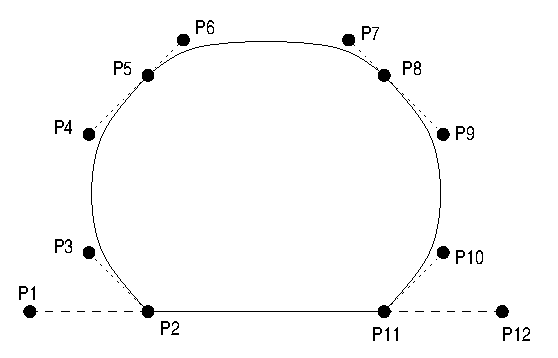
\includegraphics[scale=1.0]{outlines.eps}
\hfill\break
\vskip3mm
\hrule\vskip3mm\small
\caption{\label{figure:generaloutline}The outline of a fictive character.} 
\end{figure}
We assume that scaling, grid fitting and hinting has already been carried out.
Then, the outline is given by set of points $P_i$ and segments connecting those
points. There are:
\begin{itemize}
\item Move-segments (type = \verb+T1_PATHTYPE_MOVE+): These are straight
  segments which cause the current position to be displaced by some offset.
  Since the starting point of a segment is always implicitly the current
  point, only one argument is needed, $P_{dest}$, the destination point. In
  the figure, $P_1$--$P_2$ and $P_{2}$--$P_{12}$ are Move-segments. In this
  simple case they displace from the characters origin to some starting point
  of the outline and from the ending point of the outline to the point where
  the next character would have to be placed (the horizontal escapement). 
\item Line-segments (type = \verb+T1_PATHTYPE_LINE+): These are part of the
  path to be filled later. In analogy to the Move-segment, one argument,
  $P_{dest}$, is required for Line-segments. In the figure, $P_{11}$--$P_2$ is
  a Line-segment.
\item Bezier-segments (type = \verb+T1_PATHTYPE_BEZIER+): These are curve
  segments. Their shape is defined by a starting point (always the current
  point here), an ending point $P_{dest}$ and two control points $P_B$,
  $P_C$. These four points are the parameters of what is called a third order
  Bezier spline.\footnote{The mathematical defining equation represents a
    special case of a Bernstein polynom which was exploited by {\sc Bezier} in
    the context of solid modeling. The curve especially has the property that
    it may be approximated efficiently by straight line segments in a few
    iterations.} The resulting curve has the following 
  properties:
  \begin{itemize}
  \item It starts at the first point $P_{current}$.
  \item It ends at the fourth point $P_{dest}$.
  \item The line that goes through the points $P_{current}$ and $P_{B}$ is the
    tangent to the curve from the right side at the starting point $P_{current}$.
  \item In analogy, the line that goes through the points $P_{C}$ and
    $P_{dest}$ is the tangent to the curve from the left side at the ending
    point $P_{dest}$.
  \item The resulting curve will be enclosed completely by the convex area
    that is defined by connecting the definition points with straight line
    segments.
  \end{itemize}
  Our fictive character outline in figure \ref{figure:generaloutline}
  has three Bezier-segments, $P_{2}$--$P_{3}$--$P_{4}$--$P_{5}$,
  $P_{5}$--$P_{6}$--$P_{7}$--$P_{8}$ and
  $P_{8}$--$P_{9}$--$P_{10}$--$P_{11}$. Notice that it is easily possible to
  achieve a smooth tangent transition from one curve-segment to the next by
  choosing the involved points from a straight line.
\end{itemize}
For Type 1 fonts in general, the following rules for interpreting coordinate
specifications hold:
\begin{itemize}
\item All point specifications are relative to the {\em current
    point}. 
\item For Bezier-segments, $P_{B}$, $P_{C}$ and $P_{dest}$ all are relative to
  $P_{current}$.
\item Initially, i.e. when a character outline is started, the current point
  is at the origin $(0,0)$ of the character.
\end{itemize}
Additionally, for this special rasterizer implementation, the following terms
apply: 
\begin{itemize}
\item The vertical coordinate is---in contrast to PostScript---inverted, i.e.,
  the $y$-axis points down. 
\item Once hinted and gridfitted, the outline point coordinates are described
  in {\em fractional pixels}. A ``fractpel'' is of type \verb+long+ and
  describes the location in $2^{16}$th fractions of a pixel. To convert from
  pixel to fractional pixel and vice versa, the macros
  \verb+T1_TOPATHPOINT(p)+\index{\verb+T1_TOPATHPOINT()+} and
  \verb+T1_NEARESTPOINT(fp)+\index{\verb+T1_NEARESTPOINT()+} are provided. 
\end{itemize}

Before describing the functions for retrieving outlines the format in which
outlines are presented in C will be described. A point specification is done
in the following structure:  
\begin{verbatim}
typedef struct {
  long x;
  long y;
} T1_PATHPOINT;
\end{verbatim}
\verb+x+ and \verb+y+ are fractional pixels as described above.

An outline is represented by a linked list of structures which describe path
segments of the type described above.
Line- and Move-segments are described by the following structure:
\begin{verbatim}
typedef struct pathsegment {  
  char type;                
  unsigned char flag;       
  short references;         
  unsigned char size;       
  unsigned char context;    
  struct pathsegment *link; 
  struct pathsegment *last; 
  T1_PATHPOINT    dest;     
} T1_PATHSEGMENT;
\end{verbatim}
\verb+type+ is either \verb+T1_PATHTYPE_MOVE+ or
\verb+T1_PATHTYPE_LINE+. \verb+flag+, \verb+references+, \verb+size+ and
\verb+context+ are internally used by the rasterizer. \verb+link+ is a pointer
to the next segment structure or \verb+NULL+ in case it is the last structure
in the list. Finally, the \verb+last+-entry is a pointer to
the last structure in the linked list. \verb+last+ is only set in the first
segment and is reset to \verb+NULL+ in the remaining segment structures. 
A Bezier-segment is described by the following structure:
\begin{verbatim}
typedef struct bezierpathsegment {
  char type;              
  unsigned char flag;     
  short references;       
  unsigned char size;     
  unsigned char context;  
  T1_PATHSEGMENT *link;   
  T1_PATHSEGMENT *last;   
  T1_PATHPOINT    dest;   
  T1_PATHPOINT    B;      
  T1_PATHPOINT    C;      
} T1_BEZIERSEGMENT;
\end{verbatim}
Obviously, the format is identical to that for straight path segments, extended
by the entries \verb+B+ and \verb+C+ which specify the control points as
described earlier in this subsection.
The common return type for the outline retrieving functions is a pointer to 
\verb+T1_OUTLINE+, which is in fact identical to \verb+T1_PATHSEGMENT+. This
purely for convention. Although it is quite unlikely, an outline might start
with a Bezier-segment. To access Bezier-segment elements, a cast must be used.


\subsubsection{Using Outlines}
\label{usingoutlines}%
\tonelib\ provides three functions for retrieving outlines. The first is  
\precorr
\begin{verbatim}
 T1_OUTLINE *T1_GetCharOutline( int FontID, char charcode,
                                float size, T1_TMATRIX *transform)
\end{verbatim}\index{\verb+T1_GetCharOutline()+}\postcorr
The meaning of the arguments is as in the \verb+T1_SetChar()+-function. 
Notice that the size specification is also required here. Outlines are, by
their nature in Type~1, generally defined in a $1000\times 1000$ grid and then
scaled down by the fontmatrix to 1 bp. The space is known as the
charspace. The reason for specifying a size at this place, instead of scaling
the outline later, is, that hinting is performed according to the scaled
outline. The returned outline is then hinted for the given size. If necessary,
it may still be scaled later.

The outline for a complete string can be retrieved by
\precorr
\begin{verbatim}
 T1_OUTLINE *T1_GetStringOutline( int FontID, char *string, int len, 
                                  long spaceoff, int modflag,
                                  float size, T1_TMATRIX *transform)
\end{verbatim}\index{\verb+T1_GetStringOutline()+}\postcorr
The meaning of the arguments is as in \verb+T1_SetString()+.

Finally the ``outline'' for a displacement is available by the function
\precorr
\begin{verbatim}
 T1_OUTLINE *T1_GetMoveOutline( int FontID, int deltax, int deltay, int modflag,
                                float size, T1_TMATRIX *transform)
\end{verbatim}\index{\verb+T1_GetMoveOutline()+}\postcorr
This function is intended to be used for concatenation of outlines. It needs
all the arguments because some quantities which are given on the font level
are required for constructing the outline. \verb+deltax+ and \verb+deltay+ are
the horizontal and vertical displacement measured in charspace units. From the
\verb+modflag+-argument, especially the underlining parameters are
evaluated. Although $x$- and $y$-displacement may be specified, the resulting
outline is still subject to scaling with \verb+size+ and transformation
according to \verb+transform+. 

Arbitrary outlines may be concatenated by using the function
\precorr
\begin{verbatim}
 T1_OUTLINE *T1_ConcatOutlines( T1_OUTLINE *path1,
                                T1_OUTLINE *path2)
\end{verbatim}\index{\verb+T1_ConcatOutlines()+}\postcorr
Notice that this concatenation is done with high precision so that we can
expect that visual artefacts are reduced to a minimum (remember figure
\ref{figure:whyoutlines}). 

Scaling of outlines is done by the function
\precorr
\begin{verbatim}
 T1_OUTLINE *T1_ScaleOutline( T1_OUTLINE *path, float scale)
\end{verbatim}\index{\verb+T1_ScaleOutline()+}\postcorr
\verb+T1_ScaleOutline+ does nothing more than linearly scaling the coordinate
data with \verb+scale+ and storing the result in fractional pixels. No care is
taken for hinting (see above).

An outline may be duplicated using the function
\precorr
\begin{verbatim}
 T1_OUTLINE *T1_CopyOutline( T1_OUTLINE *path)
\end{verbatim}\index{\verb+T1_CopyOutline()+}\postcorr
This is a direct entrypoint into the rasterizer. It works by allocating and
duplicating each segment of \verb+path+. This function may be useful if one
wants to do several things with one outline because the process of filling an
outline also consumes that outline.

An outline that that a user decides not to fill can be destroyed by the
function 
\precorr
\begin{verbatim}
 void T1_FreeOutline( T1_OUTLINE *path)
\end{verbatim}\index{\verb+T1_FreeOutline()+}\postcorr
It iterates through the segment list and frees each segment.
This must not be done after filling an outline because the filling process
consumes the outline!

Finally, there are two functions that produce glyphs from outlines, namely
\precorr
\begin{verbatim}
 GLYPH *T1_FillOutline( T1_OUTLINE *path, int modflag)
\end{verbatim}\index{\verb+T1_FillOutline()+}\postcorr
and
\precorr
\begin{verbatim}
 GLYPH *T1_AAFillOutline( T1_OUTLINE *path, int modflag)
\end{verbatim}\index{\verb+T1_AAFillOutline()+}\postcorr
Their usage does not need any explanation. The value of \verb+modflag+ is
required for {\em Right-To-Left} typesetting. If the bit
\verb+T1_RIGHT_TO_LEFT+ is set, the dimension of the glyph are recomputed
accordingly. All other bits from \verb+modflag+ are ignored such that in the
usual case of {\em Left-To-Right} typesetting simply 0 can be specified.
While \verb+T1_FillOutline()+ produces bitmaps of depth 1,
\verb+T1_AAFillOutline()+ produces antialiased bytemaps of the current
graphics depth. It should be mentioned that Smart Antialiasing (see
\ref{smartantialiasing}) does not work with this function. The reason is that
\tonelib\ has no notion of the quantity ``size'' when it gets the outline to
process. Hence, Smart Antialiasing can't work in this case. As noted above,
the outline is consumed by the filling functions so that there is no need to
free it explicitly.

 
\subsubsection{Manipulation of Outlines}
\label{outlinemanipulation}%
\tonelib\ provides some limited further functionality to process
outlines. First of all, a user would expect a character to be defined in a
coordinate system in which $x$ points to the right and $y$ points up. Further,
a representation of the glyph where all points are specified in absolute
coordinates would be advantageous for manipulating outline-points. This is
because most transformations, linear or nonlinear, need to have an absolute
$x$-value to compute an $y$-value or vice versa. The function
\precorr
\begin{verbatim}
 void T1_AbsolutePath( T1_OUTLINE *rpath)
\end{verbatim}\index{\verb+T1_AbsolutePath()+}\postcorr
does exactly what has been described just before, (a) conversion of relative
coordinates into absolute coordinates and (b) inverting the
$y$-direction. 

Once a path has been converted into an absolute path, it is
suitable for possibly nonlinear manipulation.\footnote{A linear manipulation
  of path points would rather be realized using the transformation matrices as
  described in \ref{transformations}.}
As an example of what can be done, have a look at figure \ref{figure:manipulation}. 
\begin{figure}[t]
\hfill
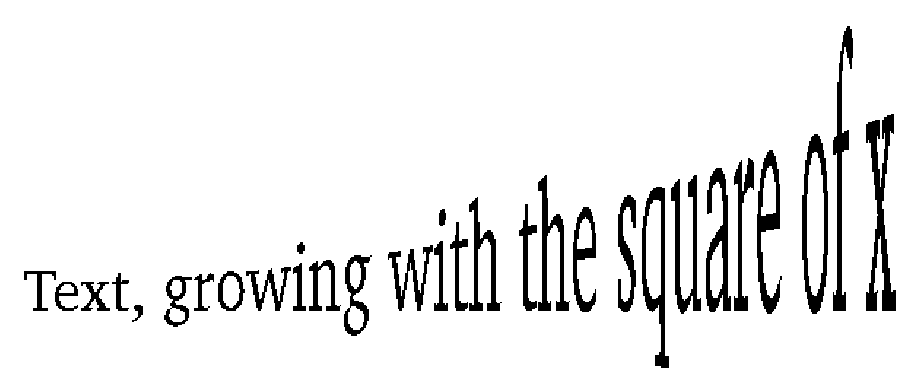
\includegraphics[scale=1.0]{manipulate.eps}
\hfill\break
\vskip3mm
\hrule\vskip3mm\small
\caption{\label{figure:manipulation}A string with nonlinearly scaled coordinates.} 
\end{figure}
The string displayed has been generated by essentially applying the
transformation $y'= y(1+cx^2)$, with appropriate $c$. To allow such
transformations by the user, \tonelib\ provides the function
\precorr
\begin{verbatim}
 void T1_ManipulatePath( T1_OUTLINE *path,
                         void (*manipulate)(long *x,long *y, int type))
\end{verbatim}\index{\verb+T1_ManipulatePath()+}\postcorr
Here, \verb+path+ should be an absolute path as described above. Notice that
\tonelib\ has no way to check whether the path is relative or absolute, this
is in the responsibility of the user. The second argument is a pointer to a
function that has a return type of \verb+void+ and that expects three
arguments: two pointers to \verb+long+-values one integer \verb+type+.
\verb+T1_ManipulatePath()+ works by iterating through all outline points of
\verb+path+ and calling the function \verb+*manipulate()+ for each outline
point. When the function \verb+*manipulate()+ is called, \verb+x+ and \verb+y+
are pointers to the $x$- and $y$-coordinates respectively of the outline point
to be processed. That way, \verb+*manipulate()+ can alter the outline
points arbitrarily. The \verb+type+-argument will be set to the segment type
by \verb+T1_ManipulatePath()+. As described earlier, the segment type can be
one of \verb+T1_PATHTYPE_MOVE+, \verb+T1_PATHTYPE_LINE+ and
\verb+T1_PATHTYPE_BEZIER+. Of course, the function \verb+manipulate()+ has to
be written by the user. To make it clear, we consider a function which
stretches an outline horizontally by 1.5. The code fragment for this could be:
\begin{verbatim}
     .
     .
     .
void h_stretch( long *x, long *y, int type)
{
  double dx;

  dx=(double)*x;
  dx *=1.5;       /* scale x coordinate by 1.5 */
  *x=(long)dx;
}
     .
     .
     .
T1_OUTLINE *path=NULL;
path=T1_GetStringOutline(FontID,(char *)SomeString,
                         0,0,T1_KERNING,20.0,NULL);
T1_AbsolutePath( path);
T1_ManipulatePath( path, &h_stretch);
T1_RelativePath( path);
glyph=T1_FillOutline( path, Modflag);
     .
     .
     .
\end{verbatim}

As the example above already has shown, an absolute path, manipulated or not,
must converted back to a relative path before it finally can be interpreted by
the rasterizer. This conversion is done using
\precorr
\begin{verbatim}
 void T1_RelativePath( T1_OUTLINE *apath)
\end{verbatim}\index{\verb+T1_RelativePath()+}\postcorr
As already mentioned with respect to \verb+T1_AbsolutePath()+, \tonelib\ cannot
check whether the \verb+path+ specified is really absolute. The user has to 
take care for this.

A few general comments about manipulating paths are appropriate. Although the
mechanism implemented by \verb+T1_ManipulatePath()+ allows arbitrary
manipulation of path points, one must be very careful in doing so. Figure
\ref{figure:outlineproblems} exhibits some of the problems that may arise. A text
string aligned to a sine function is displayed.
%- parameters of figure: string:   Text aligned along a sine wave function
%                        size:     50
%                        kerning   on
\begin{figure}[t]
\hfill
a) 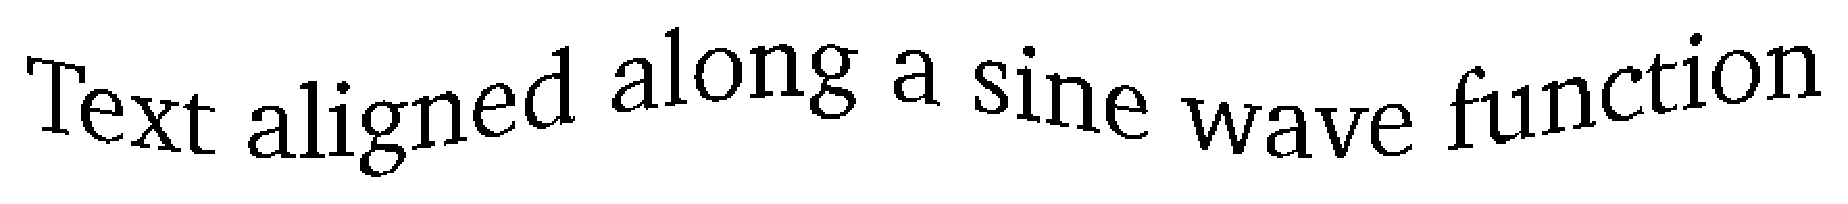
\includegraphics[scale=0.5]{outlineproblems1.eps} % period=500, 
\hfill\break

\hfill
b) 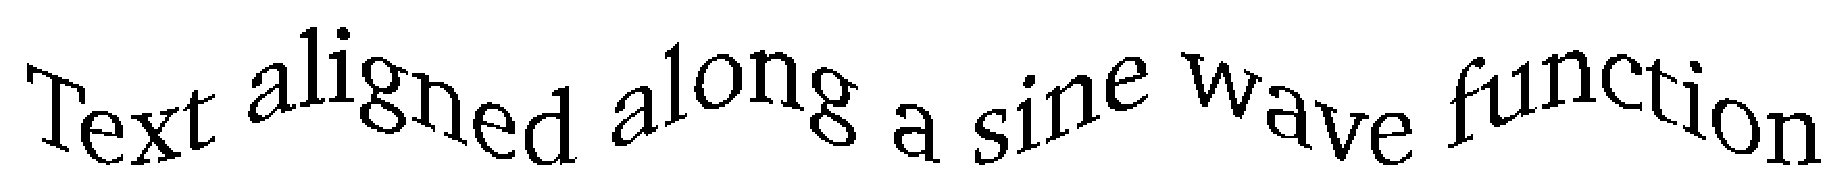
\includegraphics[scale=0.5]{outlineproblems2.eps} % period=200
\hfill\break

\hfill
c) 
\includegraphics[scale=0.5]{outlineproblems3.eps} % period=100
\hfill\break

\hfill
d) 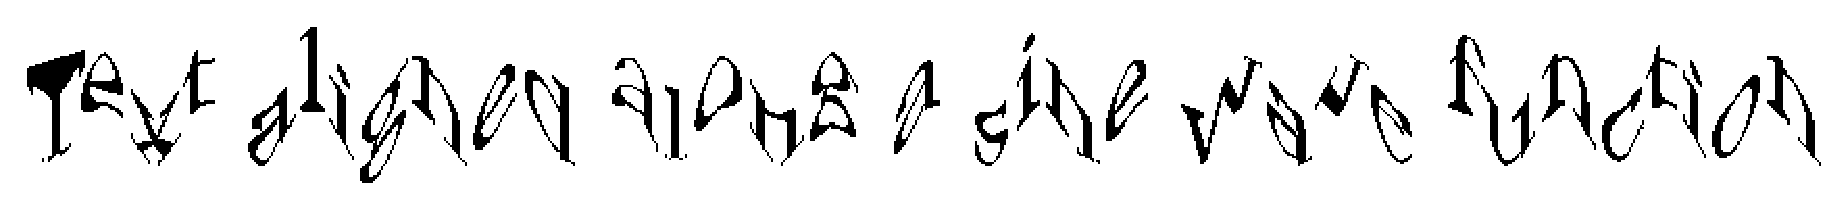
\includegraphics[scale=0.5]{outlineproblems4.eps} % period=50
\hfill\break

\hfill
e) 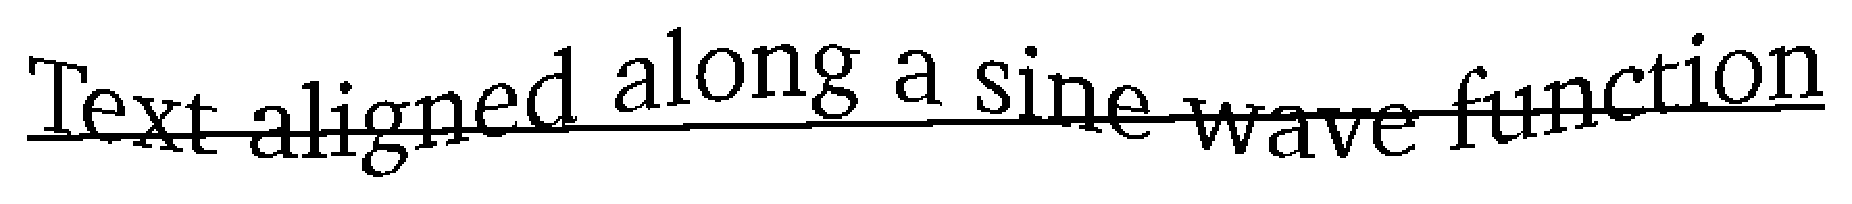
\includegraphics[scale=0.5]{outlineproblems5.eps} % period=500
\hfill\break
\hrule\vskip3mm\small
\caption{\label{figure:outlineproblems}The string ``Text aligned along a sine wave
  function'' using a period of (a) 500, (b) 200, (c) 100, (d) 50 pixels and
  (e) again 500 pixels with underlining. The sine amplitude was 30 pixels 
  (in screen resolution).} 
\end{figure}
In part (a), a pleasing smooth text flow is shown and this also applies for
(b) where the period of the sine has been reduced to 200 pixels. In (c), where
the period has been reduced to 100 pixels, some artefacts already show up. For
example, the top bar of the uppercase ``T'' has noticeable variance in
thickness. In (d), where the period has been reduced again, the result is
hardly readable. Another artefact appears in figure
\ref{figure:outlineproblems} (e): since the underlining rule is defined by
four points only, these points and nothing else is transformed with the result
that the out coming line is still straight and not curved as we would
like. From this discussion we conclude, that such transformations can only be done
with reasonable results if the maximum distance between the outline points of
a shape is small compared to the variance of the outline points that the
transformation results in. This rule, although being very fuzzy and
non-mathematical, should give a good estimation of which transformations are valid. 

Another completely independent topic is that, at the level where \tonelib\ 
provides outlines, their representation is strictly descriptive with respect
to points and their connections. There are no such things like 
\verb+closepath+-segments which would take care that a path is really closed,
no matter what the transformation had been. This means, that identical points
$P_1 = P_2$ have to be transformed to identical points $P_1'=P_2'$, no matter
where they appear in the outline. However,
if the transformation is done by by a function $(x',y')=f(x,y)$ as suggested,
this should never be a problem.

Finally, one should remember that all computations in the user function
\verb+manipulate()+ have to be done in units of fractional pixels, rather than in
pixels. When designing a sine wave as in figure \ref{figure:outlineproblems},
this must be taken into account with respect to periodicity.

\subsection{Logical Fonts}
\label{logicalfonts}%
It sometimes may be necessary to have a font and an extended or slanted
variant simultaneously. To enable such configurations without needing to
declare the fonts two or even more times in the font database file, 
\tonelib\  provides the function 
\precorr
\begin{verbatim}
 int T1_CopyFont( int FontID)
\end{verbatim}\index{\verb+T1_CopyFont()+}\postcorr
It copies the top level data structure of the font given by \verb+FontID+ to
another location. The newly created font refers in fact to the same 
physical memory as the font \verb+FontID+ as far as Type 1 and AFM data are
concerned. However, no size specific data is copied from font \verb+FontID+,
you can thus do with the new font whatever you want to. It will get its own
size-specific memory area when the first bitmap is generated using its ID.

It is also possible to reencode a copied font without affecting the
original font. This is possible because a logical font gets its own
mapping tables. This allows configurations with one font at different
encodings simultaneously.

In order to keep track that another font is referring to data from
font \verb+FontID+, a reference counter is managed for every font. The
reference counter for font \verb+FontID+ is incremented after a call to
\verb+T1_CopyFont()+. 

If the font \verb+FontID+ is not loaded into memory, the function returns $-1$.

Only {\em physical} fonts---those fonts defined in the font database
file or added via \verb+T1_AddFont()+---may be copied to another
font. If a user tries to copy a font 
which is already logical, the function returns $-2$.

If no memory is available for the new font the function return $-3$. But
this should not happen. 

If all goes the right way, \verb+T1_CopyFont()+ returns an integer---lets call
it \verb+new_ID+---which is from now on a valid font identification number.

\subsection{Missing or Invalid AFM Files}
\label{missingafmfiles}%
\tonelib\ heavily relies on AFM information every time the relative position
of bitmaps is of importance. Because AFM information is of high resolution,
accumulating positioning errors are avoided in contrast to what the X11 text
drawing functions do. On the other hand, there are many freely available
Type~1 font programs that come without AFM files. This problem has been
addressed in \tonelib\ 0.5. \tonelib\ is now able to generate AFM information
on the fly and it even can generate AFM files from Type 1 font files.

\subsubsection{Remarks on AFM Files}
\label{remarksonafmfiles}%
Information in AFM files is only relevant for placing character glyphs but not
for rasterizing. The metric values are based on the same coordinate system as
used in Type 1 font files, the so called {\em charspace coordinate system}. 
One unit is $1/1000 \mbox{bp}$ when a font is not scaled or scaled to 1~bp,
respectively. 

Information in AFM files can divided into several groups:
\begin{enumerate}
\item {\em Global Font Information:} This information is generally not needed
  to place characters. Furthermore, most of this information is also
  contained in a Type 1 font file itself. This area is thus of marginal
  importance for \tonelib. 
\item {\em Character Width's and Bounding Boxes:} These both are crucial for
  accurately placing the character glyphs. Fortunately, these are dimensions
  are exactly defined by the character outlines themselves. It is thus
  possible to compute them spending some computational effort.
\item {\em Ligature Information:} For \ae sthetic reasons, certain character
  groups are often replaced by ligatures and a font file may define several
  ligatures. It is however not intuitively clear what character groups should
  be replaced by what ligatures.\footnote{Well, at least not without some
    expert knowledge like ``I know this ligature's name is `f{}i', so I
  replace  every series of `f' and `i' with it.''}
  Fortunately, ligatures are not crucially needed for quality typesetting.
\item {\em Pair Kerning Information:} This information is quite important for
  \ae sthetic reasons but it is entirely independent from the outline
  descriptions and can thus not be extracted from a font file.
\item {\em Track Kerning Information:} This information gives hints of how to
  typeset text generally closer or wider at varying point sizes. 
  \tonelib\ does not use track kerning
  information and I personally do not consider using track kerning a good
  typographical style. 
\item {\em Composite Character Data:} This is needed to construct characters
  from two single characters. Typical examples are accented
  characters. \tonelib\ currently does not deal with composite
  characters. Most of the composite characters needed are already existent
  internally. 
\end{enumerate}
To come to a conclusion, for our purposes it is sufficient to generate the
characters' widths and their bounding boxes and we have all information we
need to construct string glyphs.

\subsubsection{Generation of AFM Information}
\label{generatingafminfo}%
Next lets consider how to generate the AFM information. It is a series of
entirely independent steps:
\begin{itemize}
\item When we generate AFM information, we want to do this once and forever
  when the font is loaded. Consequently all characters, have to be examined,
  not only those that are currently encoded. 
  We start by fetching all character names the font defines. This done with
  \verb+T1_GetAllCharNames()+ (see \ref{otherinformation}). This yields a list
  of possibly more than 256 character names.
\item Each of the character addressed by the names above is now rastered at
  size 1000~bp. By rastering at 1000~bp we match exactly the charspace
  coordinate system which the character outline descriptions are
  based on. Width and bounding box are easily examined and saved at
  appropriate places. 
\item The kerning pair area and ligatures are explicitly set to zero.
\end{itemize}
At the end of this procedure, there is a data area identical to what would
have been built when reading an AFM file without kerning-section and ligature
specifications.  

The decision of building AFM data is done on the fly without any user
interaction. Here is what happens on the metrics-area when loading a font:
\begin{itemize}
\item \tonelib\ tries to open an AFM file reading metrics and kerning pair
  information. 
\item If this does not succeed, it tries to rescan the AFM file in a {\em
    sloppy} way, only requesting metrics information.
\item If this fails too, metrics information is generated on the fly as
  described above.
\end{itemize}
It should be noted that generating metric information the way described above
takes significant amount of time since every character has to be rastered at
1000~bp.

%~derekn
If the \verb+T1_NO_AFM+ flag is passed to \verb+T1_InitLib()+,
\tonelib\ will neither attempt to open AFM files nor generate AFM
information.  This is useful to speed up applications which do not
need the metrics data. However, this slows down access to certain features,
mostly related to the string processing functions, and completely disables the
features that only are contained in AFM files (like kerning and ligatures).

Obivously, the \tonelib\ functions that use
the AFM data will not work correctly in this case and should not be
used.
%~derekn

\subsubsection{Writing AFM Files}
\label{writingafmfiles}%
In order to reduce the situations where AFM data has to be generated on the
fly, \tonelib\ provides the following function:
\precorr
\begin{verbatim}
 int T1_WriteAFMFallbackFile( int FontID)
\end{verbatim}\index{\verb+T1_WriteAFMFallbackFile()+}\postcorr
It writes an AFM file for the font identified by \verb+FontID+. This is done
executing the following steps:
\begin{enumerate}
\item The AFM filename is constructed by taking the fontfilename, cutting off
  the extension and appending \verb+.afm+.
\item A pointer array of size $256 + n$, where $n=\mbox{number of
  characters}$, is
  allocated and set to NULL. The leading 256 entries are reserved to point to 
  encoded
  characters' metrics. The remaining entries are intended to point to metrics
  of unencoded characters. We see that this is a worst case speculation: The
  pointer array is large enough for the extremely unusual case that no
  characters are encoded. 
\item Next the function steps through all character names and gets their
  encoding index $i$. If $i\geq0$, the character is encoded and the $i$th
  pointer element in the array is set to point to the metrics of this
  character. If $i=-1$, the character is not encoded and the lowest unused
  pointer in the second area is set to point to the metrics of this character.
\item Next the AFM file is opened and the header information as well as a
  comment by \tonelib\ are written. There are 5 entries that are not trivially
  to extract from the font file: \verb+Ascender+, \verb+Descender+,
  \verb+XHeight+, \verb+CapHeight+ and \verb+EncodingScheme+. Their
  discussion is deferred to later in this section.
\item After the header, the metrics information is written in the format
  required for AFM files. This is done by stepping through the pointer array
  until the first NULL pointer in the unencoded characters' area is
  reached. 
\end{enumerate}
The result is a list of char-dimensions entries which is leaded by the encoded
characters in ascending order of their encoding index, followed by a list of
unencoded characters in alphabetical order. 

As seen above, the current encoding takes influence on the order the
characters appear in the AFM file. One should thus not produce AFM files from
reencoded fonts, although this is possible. This yields non-standard AFM files
and gives no performance gain, even not when used with \tonelib.

The entry \verb+EncodingScheme+ is not always contained in the fontfile
itself. It is generated by comparison between encodings. \tonelib\ has only one
builtin encoding, \verb+AdobeStandardEncoding+, which
is recognized. Every further encoding, defined
by the font itself or applied by a user, is always marked as
\verb+FontSpecific+. 

The entries \verb+CapHeight+, \verb+XHeight+ \verb+Ascender+ and
\verb+Descender+ are not fully determined by a Type 1 font file
although they are existent with high probability. As rough definitions
can be considered:
\begin{itemize}
\item \verb+CapHeight+: The height a capital `H' reaches to.
\item \verb+XHeight+: The height a lower case `x' reaches to.
\item \verb+Ascender+: The height a lower case `d' reaches to.
\item \verb+Descender+: The depth a lower case `p' reaches down.
\end{itemize}
It is obvious that these definitions make only sense in certain font
definitions. For example, a musical notation font might not necessarily
define an ascender since no capital letters are provided. 

In the Type 1 notion these dimensions are referred to as top alignment
and bottom alignment values respectively. The corresponding alignment
``zone'', i.e., an interval, is defined by the alignment height and a
corresponding overshoot position. The alignment zones are specified in
the BlueValues array for top alignment zones and the OtherBlues
array for bottom alignment zones. A Type 1 font may define up to 7 top
alignment zones and 5 bottom alignment zones. It is unfortunately not
defined which of these alignment zones refer to \verb+CapHeight+,
\verb+XHeight+, \verb+Ascender+ and \verb+Descender+. 

\tonelib\ tries to get out of this dilemma by making a best guess:
\begin{enumerate}
\item For each of the characters `H', `x' and `d' it fetches the
  largest y-value and compares the result with each alignment zone in
  the BlueValues array. The alignment zone closest to the observed
  character dimension is assumed a candidate for the respective
  quantity. 
\item It checks whether the difference between the alignment zone just
  selected and the character dimension is within a certain tolerance
  area. This tolerance width is $\pm 30$ charspace units. If the
  result is positive, the quantity in question is assigned the
  numerical value of the standard height (not the overshoot) of this
  alignment zone. Since we are currently considering top
  alignment zone, this will always be the lower value. 
\item If the value is out of tolerance or the font even does not
  define the character, the corresponding entry in the AFM file is left
  out.
\item A comparable procedure is then done for \verb+Descender+, this
  time examining the OtherBlues array.
\end{enumerate}
Note that if the values do not seem to be correct, the corresponding
lines can be removed from the AFM file without doing any harm. These
entries are optional only.

\verb+T1_WriteAFMFallBackFile()+ can indicate  a number of error
conditions by returning appropriate values. These are:
\begin{itemize}
\item \verb+0+: No error occurred, AFM file was successfully written.
\item \verb+-1+: The AFM data for the font in question has been
  generated by reading an AFM file, there is no need to generate a new
  one. If you really want to force an AFM file to be written, take
  care that \tonelib\ does not find an AFM file when loading the
  font. 
\item \verb+-2+: The font in question is not loaded.
\item \verb+-3+: The font in question is loaded but AFM data has not
  been generated. This definitely is an error condition because it
  indicates not all characters of the font could be rastered, either
  because the font file is damaged or because there were 
  insufficient system resources. In any case the application should
  generate a logfile and this file should be examined.
\item \verb+-4+: The AFM file could not be opened. This could be a
  permission problem or something else. The file is always opened in
  the current working directory.
\item \verb+-5+: The file has successfully been opened but there was
  an error writing to the file.
\item \verb+-6+: A memory allocation error occurred. This should not
  happen because it indicates there are no system resources. 
\end{itemize}


\subsection{Error Handling}
\label{errorhandling}
Although every function usually returns meaningful values, there are
situations where indicating an error via the return value is not possible. For
example, requesting a charspace bounding box from a char of a font which is not
loaded will return a bounding box containing all zeroes. This cannot be
considered an error-condition since for characters like ``space'' it is
correct to return a bounding box containing all zeroes. Furthermore, there's no
consistent scheme which value should indicate what type of error. In order to
allow a unified error handling in applications, the global variable
\verb+T1_errno+ has been introduced. 

The functionality of \verb+T1_errno+ is analogous to that of the global
\verb+errno+ in C programs. \verb+T1_errno+ is once set to 0 when the library
is initialized and never reset by any \tonelib-function. It is set to specific
values when specific types of errors appear. An application may then act
appropriately and reset \verb+T1_errno+.
The errors that might appear can be roughly split into three categories as
described below.

\subsubsection{Type 1 Font File Scan-Errors}
These types of errors can only appear at the time a font file is loaded.
These kinds of errors are indicated by negative values:
\begin{itemize}
\item \verb+T1ERR_SCAN_FONT_FORMAT+ (-5): A Multiple Master Font was attempted
  to be loaded. These are not supported by \tonelib.
\item \verb+T1ERR_SCAN_FILE_OPEN_ERR+ (-4): This value indicates that the Type
  1 font file could not be opened by the parser. It usually does not mean that
  the file does not exist because this problem would have shown up at the time
  the font database had been built. It is more likely a permission problem.
  Anyhow, the C library variable \verb+errno+ should be examined for getting
  an idea of what the problem was.
\item \verb+T1ERR_SCAN_OUT_OF_MEMORY+ (-3): A Type 1 font program required
  more than 262144 bytes of VM. This is a limit imposed by \tonelib\ because
  it usually means there goes something wrong. Typical values of VM
  consumption are between 30000 and 60000 bytes depending on the fonts'
  complexity. If this limit really does not suffice the constant
  \verb+MAXTRIAL+ (defined in \verb+lib/type1/fontfcn.c+) may be set to some
  larger value. 
\item \verb+T1ERR_SCAN_ERROR+ (-2): An error occurred during scanning the font
  file. It usually means that the font file is damaged or does not comply to
  the conventions of Type 1 font files. For example, an encountered token might
  have been too long. Another reason could be, a literal name follows a literal
  name where a number was expected. There is no way to recover from this
  error. One last resort could be to disassemble the font (e.g., using
  \verb+t1disasm+ from the \verb+t1utils+ package) and scan the resulting
  human-readable file for possible violations of the Type 1 font format
  specifications. However, some knowledge about the format is in force.
\item \verb+T1ERR_SCAN_FILE_EOF+ (-1): A premature end of file was encountered
  during parsing. The file is damaged.
\end{itemize}

\subsubsection{Path Generation Errors}
Small positive number are reserved for errors that might appear during path
construction and rasterization. 
\begin{itemize}
\item \verb+T1ERR_PATH_ERROR+ (1): An error occurred during path
  construction. The font file is most probably damaged.
\item \verb+T1ERR_PARSE_ERROR+ (2): This kind of error describes a kind of
  ``semantic'' error in the font file. A typical candidate for this is a font
  that does not define a character named \verb+.notdef+, although this is
  required by the format specification. Since under usual conditions the
  \verb+.notdef+ character is never accessed, this error would not show
  up. But if for some reason the \verb+.notdef+ has to be substituted for some
  other character the problem becomes evident.
\item \verb+T1ERR_TYPE1_ABORT+ (3): The \verb+abort()+-function of the
  rasterizer has been called. This may happen at several places during
  hinting, converting to edgelists etc. There is a certain chance that
  unfreed memory has been left. If this error appears and a logfile is used,
  an error string giving some more info is placed into the logfile.
  
  This error should not appear, normally. If it does, either the font file is
  damaged or the font contains invalid outline descriptions such as unclosed
  paths. Especially the latter is quite unlikely. Of course this error can be
  raised, when an outline has been modified manually in an invalid way and is
  then rastered (see.~\ref{outlinemanipulation}).
\end{itemize}

\subsubsection{\tonelib-Errors}
The remaining types of errors are detected by the management of \tonelib. Their
numbering starts with 10 (decimal). The list could be extended in future
releases. 
\begin{itemize}
\item \verb+T1ERR_INVALID_FONTID+ (10): An invalid font ID has been
  specified. The exact meaning of this error depends on the specific
  situation, in any case the operation requested cannot be realized with the
  identified font. Possible reasons are:
  \begin{itemize}
  \item The font ID points to a font which is not loaded and which must be
    loaded in order to perform the operation.
  \item The specified font ID is a number which is generally out of the range
    of the valid font IDs, either because it is $<0$ or because it is $>$ the
    value of \verb+no_fonts+.
  \item The library is not yet initialized so that no font ID at all is valid.
  \end{itemize}
\item \verb+T1ERR_INVALID_PARAMETER+ (11): One or more of the parameters
  specified to a function call were assigned invalid values. For example, a
  size-value specified to a rastering function must always be $>0$. Just the
  same way, \verb+T1_ConcatGlyphs()+ cannot concatenate two glyphs if one of
  them is the \verb+NULL+ pointer.
\item \verb+T1ERR_OP_NOT_PERMITTED+ (12): An operation that was not allowed
  {\em at that time} has been requested. This error could result, for example,
  if an application tries to set a new bitmap padding value after \tonelib\
  has been initialized. 
\item \verb+T1ERR_ALLOC_MEM+ (13): This error indicates that \tonelib\ ran out
  of memory and a memory allocation failed. This error should not appear.
\item \verb+T1ERR_FILE_OPEN_ERR+ (14): A file that was needed could not be
  opened by \tonelib. The file might have been necessary for reading data or
  writing data. For example, \verb+T1_WriteAFMFallbackFile()+ returns this
  value if the AFM file could not be opened for writing and
  \verb+T1_LoadEncoding()+ returns it if the encoding file specified as
  argument could not be opened. Notice that there is no indication of the
  reason why the file opening failed. The C library
  variable \verb+errno+ should be examined to analyze this further.

  It should be mentioned that \verb+T1ERR_FILE_OPEN_ERR+ is only set if a file
  operation failed which was really in force. This means that at the time a
  font is loaded a missing AFM file does not cause \verb+T1_errno+ caused to
  be set to \verb+T1ERR_FILE_OPEN_ERR+. This is because \tonelib\ can
  automatically recover from this by generating AFM information on the fly (at
  the cost of computation time).
\item \verb+T1ERR_UNSPECIFIED+ (15): This value indicates nothing apart from
  that an error occurred and this error was not one the other errors. It can
  be considered a fallback. Currently this value is set, for example, if an
  encoding file was tried to be loaded which did not specify exactly 256
  characters. 
\item \verb+T1ERR_NO_AFM_DATA+ (16): A function has been called which needs
  AFM information and AFM information is not available, either because all
  attempts to generate AFM data failed or because the flag \verb+T1_NO_AFM+
  has been specified as part of the flag for \verb+T1_InitLib()+. 
\item \verb+T1ERR_X11+ (17): An error in an X11 library function occured. Thus
  could be caused by calling a function of the X11 interface without prior
  initialization of the X11 interface via \verb+T1_SetX11Params()+.
\end{itemize}


\subsection{Other Useful Functions}
\label{otherfunctions}
This subsection describes a few functions that had not been described up to
now but which however could be useful.

\precorr
\begin{verbatim}
 int T1_CheckEndian( void)
\end{verbatim}\index{\verb+T1_CheckEndian()+}\postcorr
This function may be used to check the endianess of the hardware \tonelib\ is
running on. The return value is \verb+0+ for Little Endian and \verb+1+ for
Big Endian machines.

\precorr
\begin{verbatim}
 void T1_DumpGlyph( GLYPH *glyph)
\end{verbatim}\index{\verb+T1_DumpGlyph()+}\postcorr
This function might be useful for debugging and testing \tonelib. It dumps an
ASCII representation of the glyph pointed to by \verb+glyph+ to the standard
output. A background pixel is represented by \verb+.+ while a foreground pixel
is represented by \verb+X+. After the number of bits that correspond to the
current padding value, an empty column is inserted. See the output of the
programming example in \ref{programmingexample}. In this case the padding
values has been 16.

Note that the size of the glyph should be small enough that its padded width
does not exceed the terminals line width. Otherwise the result might become
illegible. 

\precorr
\begin{verbatim}
 void T1_DumpPath( T1_OUTLINE *path)
\end{verbatim}\index{\verb+T1_DumpPath()+}\postcorr
This function dumps a description of an outline to the standard output. It is
exclusively intended for debugging purposes.


\precorr
\begin{verbatim}
 void T1_SetRasterFlags( int flags)
\end{verbatim}\index{\verb+T1_SetRasterFlags()+}\postcorr
This function allows to enable or disable certain features of the
rasterizer. Let me emphasize that this is exclusively intended for debugging
and error tracking. The default value of \verb+flags+ is 0 which means that no
debugging output is shown and hinting is performed as suggested in the {\em Adobe
Type Font Format}. However there may arise situations where fiddling with the
\verb+flags+ might be helpful in rasterizer and font debugging. 

\verb+flags+ usually is an OR'ed combination of the following definitions:
\begin{itemize}
\item \verb+T1_IGNORE_FORCEBOLD+
\item \verb+T1_IGNORE_FAMILYALIGNMENT+
\item \verb+T1_IGNORE_HINTING+
\item \verb+T1_DEBUG_LINE+
\item \verb+T1_DEBUG_REGION+
\item \verb+T1_DEBUG_PATH+
\item \verb+T1_DEBUG_FONT+
\item \verb+T1_DEBUG_HINT+
\end{itemize}
The \verb+T1_IGNORE_...+ types allow to selectively disable hinting. They
might be useful if parts of a font are not properly rendered. For example,
substituting a font's alignment zones by the family's alignment zones might
result in visual artifacts if the values for \verb+FamilyBlues+ are not
correct. Disabling family alignment might reveal the problem in such cases.

The \verb+T1_DEBUG_...+ types produce debugging output from the intermediate
rasterizing steps. Notice that to understand this output a thorough
understanding of what happens in the rasterizer is in force. Moreover, be
prepared that thousands of lines might be written to the terminal, depending
on the particular option.

%%% Local Variables: 
%%% mode: latex
%%% TeX-master: "t1lib_doc"
%%% End: 
